% !TEX root = ../thesis.tex
\chapter{Problemanalyse}\label{ch:analyse}
In diesem Kapitel wird Smart Gardening und dessen Umfeld analysiert, um Anforderungen an ein universelles Sensor- und Aktuatorsystem für Smart Gardening zu definieren.
Dafür wird zunächst die Zielgruppe definiert und analysiert.
Anschließend werden die verschiedenen Gartenarten und -elemente aufgelistet, beschrieben und auf die verwendbaren Smart Gardening Aspekte untersucht.
Dazu gehört, wo, warum und wie Smart Gardening eingesetzt werden kann.
Aufbauend auf der Begriffsdefinition, der Zielgruppe und dem Kontext werden Anforderungen an das Smart Gardening System gestellt.
Am Ende werden die Ergebnisse der Problemanalyse zusammengefasst.



\section{Zielgruppe}
In diesem Abschnitt wird die Zielgruppe von Smart Gardening definiert und analysiert.
Smart Gardening kann von verschiedenen Gruppen mit unterschiedlichen Bedürfnissen genutzt werden~\cite{IoTFarming, SmartGardeningBeliebt}.
An erster Stelle stehen Gärtner, unterteilt in Hobbygärtner und professionelle Gärtner, wobei Hobbygärtner die primäre Zielgruppe bilden und dementsprechend bei Konflikten präferiert behandelt werden.
Obwohl Landwirte ebenfalls von Smart Gardening Lösungen profitieren können, liegt der Fokus dieser Arbeit nicht auf dieser Gruppe, und die Anforderungen sind nicht speziell auf sie zugeschnitten, sie werden nur rudimentär betrachtet.
Zu den Bedürfnissen gehören etwa die Pflege und Verschönerung des Gartens, die Generierung von Profit und die Selbstversorgung mit Nahrungsmitteln.
Aus diesen Bedürfnissen soll eine einheitliche Menge an Anforderungen an Smart Gardening abgeleitet werden.
Einige Faktoren wie die Qualität und Zuverlässigkeit der Lösungen sind für alle Zielgruppen relevant.

Viele Deutsche betreiben Gartenarbeit als Hobby und sind somit Hobbygärtner~\cite{GartenHobby}.
Dabei haben sie unter anderem ein Interesse an der Pflege und Verschönerung ihres Gartens.
Auch der Anbau von eigenem Essen ist ein häufiges Ziel~\cite{Gartenfavoriten}.
Dabei haben sie unterschiedliche Erfahrungen und Kenntnisse sowie unterschiedliche Grundvoraussetzungen in Größe und Art des Gartens.
Auch das Budget ist in vielen Fällen beschränkt, weshalb günstige Lösungen gefragt sind~\cite{GartenAusgaben}.
Hierbei ist auch die einfache Bedienbarkeit des Systems ein wichtiger Aspekt, da Hobbygärtner normalerweise weniger Erfahrungen als professionelle Gärtner haben.

\pagebreak

Professionelle Gärtner sind speziell ausgebildet und betreiben Gärtnerei als Beruf.
Hierbei gibt es verschiedene Spezialisierungen.
Zu diesen Spezialisierungen gehören Zierpflanzenbau, Obstbau, Staudengärtnerei, Baumschulen, Gemüsebau, Friedhofsgärtnerei und Garten- und Landschaftsbau, um nur einige zu nennen~\cite{Gaertnerarten}.
Alle diese Spezialisierungen pflegen Pflanzen verschiedener Arten und in verschiedenen Umgebungen wie Gewächshäusern, Gärten, Wäldern, Parks und Friedhöfen. 
Dadurch haben sie gemeinsame Anforderungen durch die Ähnlichkeit der Tätigkeiten und unterschiedliche Anforderungen durch die Diversität der Umgebungen.
Hier liegt der Fokus auf den gärtnerübergreifenden Aspekten, während die umgebungsabhängigen Aspekte im folgenden Abschnitt behandelt werden.
Durch das Ziel des Geldverdienens von professionellen Gärtnern haben sie normalerweise ein höheres Budget als Hobbygärtner zur Verfügung.
Für diese Kommerzialität ist neben der Zuverlässigkeit auch die Effizienz des Systems ein wichtiger Faktor.
Zur Effizienz gehört sowohl die Vermeidung unnötiger Arbeit als auch die Optimierung von Arbeitsabläufen.
So nimmt etwa ein automatischer Mähroboter dem Gärtner Arbeit ab, während ein intelligentes Benachrichtigungssystem den Gärtner informieren kann, wenn Frost droht und er die Pflanzen schützen sollte.
Dies optimiert seine Handlungsabläufe und spart ihm somit Zeit und sowohl indirekt als auch direkt Geld.

Eine weitere Gruppe sind Landwirte, die ebenfalls in Untergruppen unterteilt werden können.
So gibt es etwa kleine und große Landwirte mit fließendem Übergang, Viehzuchtbetriebe, Gewächshausbesitzer und Forstwirte~\cite{AgrarbetriebDefinition}.
Landwirte betreiben dabei im Allgemeinen große Flächen, weshalb die Lösungen skalierbar sein müssen.
Aufgrund des kommerziellen Interesses und großer Umsätze ist das Budget hier im Vergleich zu den anderen Gruppen noch einmal höher~\cite{UmsatzLandwirtschaft}.
Das Ziel eines Landwirts, Profite zu generieren, erreicht er dadurch, möglichst viele landwirtschaftliche Produkte zu produzieren.
Smart Gardening kann dies auf viele Arten beeinflussen, sowohl negativ als auch positiv.
Fällt etwa ein automatisches Bewässerungssystem aus, kann die Ernte beschädigt werden.
Gleichzeitig kann ein im richtigen Zeitpunkt gießendes System den Ertrag steigern, Wasser und somit Kosten sparen und die Umwelt schonen.
Daher ist neben der Zuverlässigkeit auch die Effizienz des Systems bei der Nutzung von Ressourcen, Steigerung von Erträgen und Einsparen von Arbeit ein wichtiger Faktor.
Smart Gardening Systeme, die Schädlingsbefall reduzieren und optimale Düngungs-, Bewässerungs- und Erntezeitpunkte bestimmen, können beispielsweise hierbei helfen.

Zusammengefasst besteht die Zielgruppe von Smart Gardening aus Hobbygärtnern, professionellen Gärtnern und Landwirten, wobei die Hobbygärtner die primäre Zielgruppe darstellen, die professionellen Gärtner die sekundäre Zielgruppe und Landwirte in dieser Arbeit nur rudimentär angerissen werden.
Diese haben unterschiedliche Bedürfnisse und Anforderungen an Smart Gardening Lösungen.
Im Folgenden wird das Umfeld von Smart Gardening analysiert, insbesondere die verschiedenen Gartenarten und -elemente.



\section{Kontext und Umfeld}
In diesem Abschnitt wird das Einsatzgebiet des Smart Gardening Systems analysiert.
Dieses setzt sich aus Gartenarten und Gartenelementen zusammen.
Zunächst werden die verschiedenen Gartenarten definiert und auf ihre Besonderheiten für den Einsatz von Smart Gardening untersucht.
Darauffolgend werden die Gartenelemente definiert und analysiert, wie Smart Gardening hier eingesetzt werden kann.
Zum Schluss wird ein Fazit gezogen und die Kombinationsmöglichkeiten von Gartenarten mit Gartenelementen dargestellt.

\subsection{Gartenarten}
In diesem Abschnitt werden verschiedene Gartenarten eingeführt und im Kontext von Smart Gardening analysiert.
Es gibt nicht den ,,einen Garten'', sondern viele verschiedene Varianten in unterschiedlichen Stilen.
Diese weisen üblicherweise unterschiedliche Eigenschaften und Anforderungen auf.
Daher kann hier nur eine Teilmenge behandelt werden.

Im Folgenden werden zunächst gartenübergreifende Aspekte analysiert.
Darauf folgen die nach der ungefähren Größe sortierten Gartenarten Balkongarten, Gewächshaus, Vorgarten, Kleingarten, Hintergarten, großer Garten als eine Art von Hintergarten und Landschaftsgarten.
Da auch in der Landwirtschaft Smart Gardening Anwendung finden kann, wird diese zusätzlich aufgeführt.
Für die Analyse der Gartenarten werden zunächst die Gartenarten erklärt, danach werden sie voneinander abgegrenzt und ihre Besonderheiten herausgestellt.
Zum Schluss wird betrachtet, von welchen Messungen und Automatisierungen sie profitieren können.

\subsubsection{Gartenartübergreifende Aspekte}

\begin{table}[!htb]
	\centering
	\caption[Gegenüberstellung von Gartentypen: Strom, Wasser und Internet.]{
		Gegenüberstellung verschiedener Gartentypen in den Bereichen der Stromversorgung, Wasserversorgung und Internetverbindung.
		Die folgenden Optionen beziehen sich darauf, wie häufig eine fest installierte Versorgungsmöglichkeit in einem Großteil eines Gartens verfügbar ist.
		Dabei gibt es für Strom und Wasser die Optionen \emph{selten}, \emph{teilweise} und \emph{häufig}.
		Es gibt keine guten Datenquellen für diese Einschätzungen.
		Daher basieren die Angaben für Strom und Wasser auf den Erfahrungen des öffentlich und bestellten Sachverständigen der Handwerkskammer Lübeck für das Installateur- und Heizungsbauerhandwerk \href{https://www.junghans-heizung.de/über-uns/}{Henning Junghans}.
		So kann es in einem großen Garten sein, dass Strom nur in Hausnähe verfügbar ist.
		Für Internet gibt es die Optionen \emph{PAN}, \emph{LAN} und \emph{WAN}.
		Hierbei sind die genannten jeweils die normalerweise im ganzen Garten verfügbaren Netzwerke.
		}\label{tab:gartenarten}
	\begin{tabular}{llll}
		Garten							& Strom 	& Wasser	& Internet		\\\hline
		Balkongarten					& Teilweise	& Selten	& PAN, LAN, WAN	\\
		Gewächshaus						& Selten	& Selten	& WAN			\\
		Vorgarten						& Selten	& Selten	& PAN, LAN, WAN	\\
		Kleingarten						& Teilweise	& Teilweise	& WAN			\\
		Hintergarten					& Teilweise	& Häufig	& WAN			\\
		Großer Garten					& Selten	& Teilweise	& WAN			\\
		Landschaftsgarten				& Selten	& Selten	& WAN			\\
		Konventionelle Landwirtschaft	& Selten	& Selten~\cite{BewFlaechen,BewFlaechenPresse}	& WAN
	\end{tabular}
\end{table}

Zunächst werden gemeinsame Aspekte der verschiedenen Gartenarten betrachtet, welche auf die meisten Gartenarten zutreffen.
Fast alle Gartenarten sind den Elementen ausgesetzt, wozu etwa Regen, Schnee, Wind, Sonne und Temperaturschwankungen zählen.
Diese haben Auswirkungen auf Smart Gardening Lösungen.

Ein weiterer geteilter Aspekt ist die Notwendigkeit der Versorgung mit Strom sowie die Relevanz der Versorgung mit Wasser und Internet für viele Smart Gardening Anwendungen.
Hierbei wird Strom benötigt, um die Sensoren und Aktuatoren zu betreiben.
Wasser wird beispielsweise benötigt, um automatische Bewässerungssysteme und Luftbefeuchter zu betreiben.
Internet wird benötigt, um Messergebnisse zu übertragen und das System fernzusteuern.

Dabei gibt es Unterschiede in der Verfügbarkeit dieser Versorgungsmöglichkeiten, welche in \cref{tab:gartenarten} dargestellt werden.
So wird deutlich, dass ein Smart Gardening System nicht von der Verfügbarkeit einer fest installierten Stromquelle wie einer Außensteckdose ausgehen kann.
Dies gilt für alle Gartenarten, wobei dies eine Verallgemeinerung ist und es Ausnahmen geben kann.
Ist kein Stromanschluss verfügbar, muss die Smart Gardening Lösung mit Batterien oder Akkus betrieben werden, wobei Solarzellen eine Möglichkeit sind, diese aufzuladen.
Auch auf eine fest installierte Wasserversorgung in Form eines Außenwasseranschlusses kann in den meisten Fällen nicht vertraut werden.
Wenn kein Wasseranschluss verfügbar ist, so muss das Wasser anderweitig beschafft werden, um Smart Gardening Lösungen wie automatische Bewässerungssysteme zu betreiben.
Hierfür eignen sich unter anderem Regentonnen, Wassertanks und Brunnen, die später noch genauer besprochen werden.
Für die Internetverbindung gibt es in den meisten Fällen keine Möglichkeit, auf eine LAN- oder PAN-Verbindung zu setzen.
Daher muss in solchen Fällen auf eine WAN-Verbindung zurückgegriffen werden.

Ein weiterer Aspekt, der alle Gartenarten betreffen kann, sind Schädlinge, die sich im Garten bedienen.
Zu diesen zählen Läuse, Milben, Schnecken, Mäuse, Maulwürfe, Vögel, Kaninchen und Rehe.
Diese können die Pflanzen schädigen, weshalb der Schutz der Pflanzen vor diesen wichtig ist.
Gleichzeitig können diese Tiere auch nützlich sein, wie der Maulwurf, der selbst Schädlinge frisst.
Außerdem sind einige Tiere gesetzlich geschützt nach §~44 Absatz~1 BNatSchG, wie der Maulwurf, weshalb eine angepasste und angemessene Reaktion notwendig ist.
Eine nicht invasive Detektion von Schädlingen und anderen Tieren ist hierbei unschädlich.
Auf Basis dieser Erkennung kann der Nutzer über die Tiere informiert werden, sodass er angemessen reagieren kann.
Eine weitere Reaktion kann das automatische Verjagen der Tiere sein, beispielsweise wirken verschiedene Gerüche und Töne abschreckend auf Tiere.
Bei der Wahl dieser Mittel ist darauf zu achten, dass sie die rechtlichen Rahmenbedingungen zum Tier- und Umweltschutz einhalten.


\subsubsection{Balkongarten}
\begin{figure}[!htb]
	\centering
	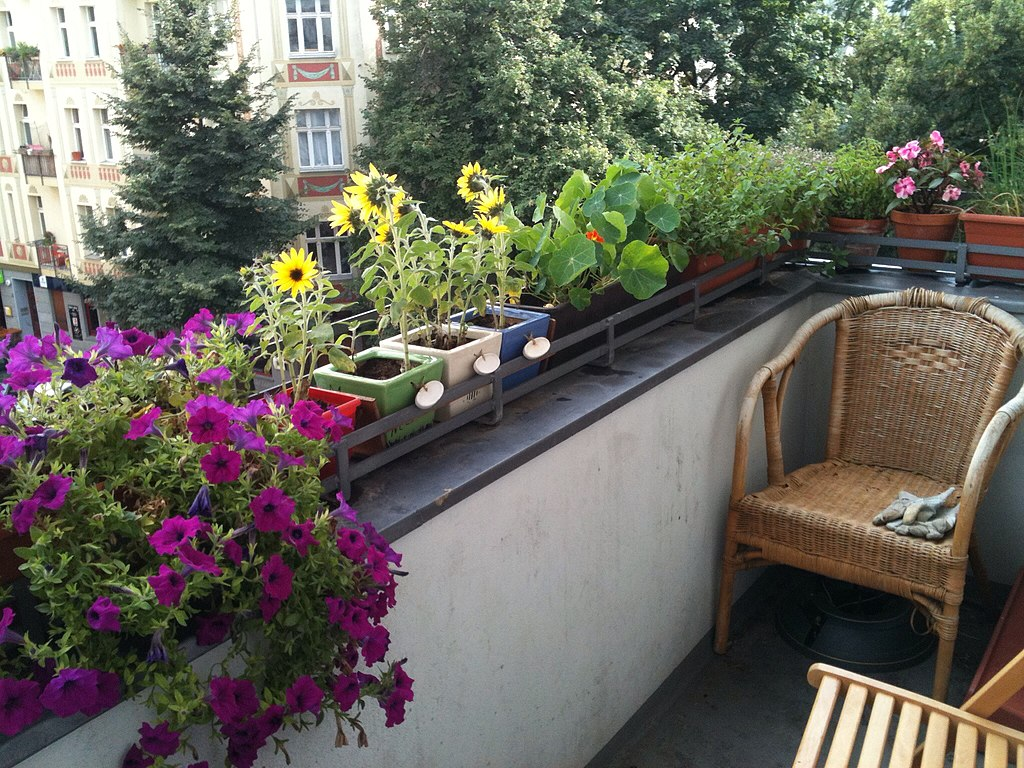
\includegraphics[width=0.5\textwidth]{images/Balkongarten.jpeg}
	\caption[Bild eines Balkongartens mit verschiedenen Balkonkästen.]{
		Bild eines engen Balkongartens mit verschiedenen Balkonkästen, in denen unterschiedliche Pflanzen wachsen.\footnotemark
		}
	\label{pic:balkongarten}
\end{figure}

\footnotetext{Bildquelle: tlcoles, \href{https://creativecommons.org/licenses/by-sa/3.0}{CC BY-SA 3.0}, via Wikimedia Commons}

Balkone sind in Deutschland weitverbreitet und viele Menschen nutzen den begrenzten Platz auf ihren Balkonen, um kleine Gärten anzulegen~\cite{VuMABalkon}.
Ein solcher ist beispielsweise in \cref{pic:balkongarten} zu sehen.
Bei diesen Balkongärten genannten Gärten kommen hauptsächlich Balkonkästen und Blumentöpfe zum Einsatz, aber auch kleine, nicht begehbare Gewächshäuser sind möglich.
Diese Gartenart zeichnet mehrere Aspekte aus.
Wie in \cref{pic:balkongarten} zu sehen, ist der Platz in vielen Fällen begrenzt, weshalb mögliche Smart Gardening Lösungen kompakt sein sollten.
Auf diesem Balkon sollte die Lösung beispielsweise nicht den Laufweg blockieren.
Als weiterer Aspekt gibt es keine Möglichkeit, Pflanzen direkt in den Boden zu pflanzen, sie müssen in Töpfen oder Kästen wachsen.
Da Töpfe und Balkonkästen Wasser schlechter halten als der Boden, ist hier eine Bewässerung besonders wichtig.
Die eben genannten Aspekte gelten analog auch für die deutlich selteneren Dachterrassen, mit dem Unterschied, dass diese meist größer sind.

\subsubsection{Gewächshaus}

\begin{figure}[!htb]
	\centering
	\includegraphics[width=0.4\textwidth]{images/Gewächshaus-Glas.jpg}
	\includegraphics[width=0.4\textwidth]{images/Gewächshaus-Folie.jpg}
	\caption[Bilder eines Glasgewächshauses und eines Foliengewächshauses.]{
		Zwei Bilder von Gewächshäusern.
		Auf dem linken Bild ist ein mittelgroßes Glasgewächshaus zu sehen.
		Es ist deutlich ersichtlich, dass es fest installiert ist, da der untere Teil gemauert und der obere Teil aus Glas ist.
		Die Dachflächenfenster können geöffnet werden.
		Die Pflanzen im Gewächshaus sind in Töpfen und Kästen gepflanzt.\\
		Auf dem rechten Bild ist ein Foliengewächshaus zu sehen.
		Dieses besteht aus einem Metallgerüst, das mit Folie bespannt ist, wobei auch die Tür aus Metall und Folie besteht.
		Abgesehen von der Tür gibt es keine beweglichen Teile.
		Die Pflanzen im Gewächshaus sind direkt in den Boden gepflanzt.\footnotemark
		}
	\label{pic:gewächshaus}
\end{figure}

Ein Gewächshaus ist eine kontrollierte Umgebung, die der Herstellung bestmöglicher Bedingungen für Pflanzenwachstum dient.
Dementsprechend kann diese Umgebung von Smart Gardening profitieren.
Es gibt kleine und große Gewächshäuser, die sowohl privat als auch kommerziell genutzt werden.
Die Anforderungen einer kommerziellen Nutzung sind dabei höher als die einer privaten Nutzung, wie eine höhere Zuverlässigkeit, da ein Ausfall zu hohen finanziellen Verlusten führen kann.

Gewächshäuser können in einfache und günstige Foliengewächshäuser sowie teure und fest verbaute Glasgewächshäuser unterteilt werden.
In \cref{pic:gewächshaus} sind beispielhaft ein Glasgewächshaus und ein Foliengewächshaus zu sehen.
Auch wenn es sich bei beiden um Gewächshäuser handelt, so gibt es doch viele Unterschiede, insbesondere bezogen auf Smart Gardening.
So ist ein Glasgewächshaus fest installiert und die Pflanzen sind in Töpfe und Kästen gepflanzt.
Ein Foliengewächshaus hingegen ist mobil und die Pflanzen sind direkt in den Boden gepflanzt.
Daraus ergeben sich unterschiedliche Anforderungen an Smart Gardening Lösungen, wobei die Anforderungen eines Foliengewächshauses denen eines Beetes ähneln.
Dies ergibt sich daraus, dass ein Foliengewächshaus praktisch ein überdachtes Beet ist, wie in \cref{pic:gewächshaus} zu sehen.
Daher fokussiert sich dieser Abschnitt auf Glasgewächshäuser.

\footnotetext{Bildquellen:\\
	Links: Vanellus Foto, \href{https://creativecommons.org/licenses/by-sa/3.0}{CC BY-SA 3.0}, via Wikimedia Commons,\\
	Rechts: Selso, \href{https://creativecommons.org/licenses/by-sa/2.5}{CC BY-SA 2.5}, via Wikimedia Commons
}

Ziel eines Gewächshauses ist es, Erträge von Pflanzen in einem geschützten Raum mit kontrollierten Bedingungen zu maximieren.
So müssen die Sensoren möglichst genau und die Aktuatoren möglichst fein regelbar sein.
Gleichzeitig ist die Umgebung besonders feucht und warm.
In einem Gewächshaus wachsen viele Pflanzen auf engem Raum, was in \cref{pic:gewächshaus} erahnt werden kann, wobei es gleichzeitig viele Parameter zu überwachen und zu steuern gibt.
So sind etwa Temperatur, Luftfeuchtigkeit, Licht, CO$_2$-Gehalt, Wasserstand und Nährstoffgehalt zu überwachen und zu steuern.
Genaueres dazu wird in \cref{sec:gartenlement-gewächshaus} erläutert.
Aufgrund des begrenzten Platzes mit vielen Sensoren und Aktuatoren ist es wichtig, dass diese nicht stören.
Gleichzeitig ist alles im Gewächshaus besser gegen die Elemente geschützt als im Freien, wo beispielsweise Regen und Wind die Sensoren und Aktuatoren beschädigen können.

\subsubsection{Vorgarten}
\begin{figure}[!htb]
	\centering
	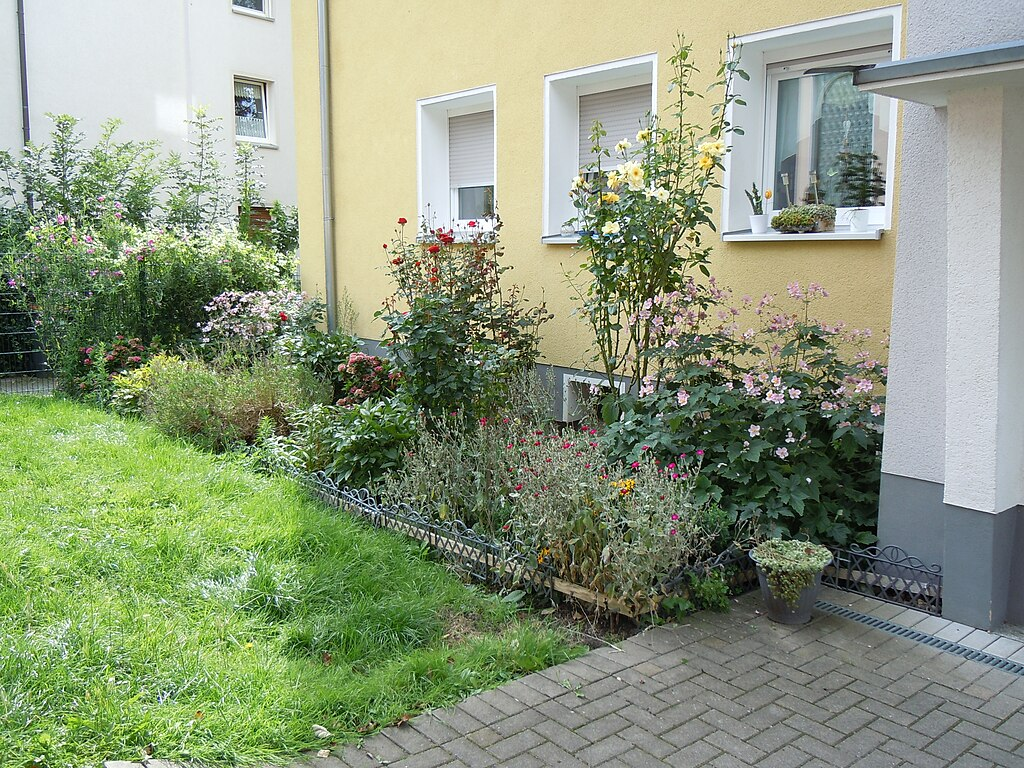
\includegraphics[width=0.5\textwidth]{images/Vorgarten.jpg}
	\caption[Bild eines typischen Vorgartens eines Mehrfamilienhauses.]{Bild eines typischen Vorgartens eines Mehrfamilienhauses.\footnotemark}
	\label{pic:vorgarten}
\end{figure}

\footnotetext{Bildquelle: Sebastian Martin Dicke, \href{https://creativecommons.org/licenses/by-sa/4.0}{CC BY-SA 4.0}, via Wikimedia Commons}

Viele Häuser weisen Vorgärten auf, insbesondere Reihenhäuser und Einfamilienhäuser, aber auch Mehrfamilienhäuser können Vorgärten haben, wie in \cref{pic:vorgarten} zu sehen.
Dieser ist meist relativ klein und dient der Verschönerung des Hauses aus der Sicht der Straße.
Demzufolge ist es wünschenswert, wenn die Smart Gardening Lösungen möglichst unauffällig sind und sich in die Umgebung integrieren lassen.
Im Beispiel des Vorgartens in \cref{pic:vorgarten} ist ein Rasen und ein Blumenbeet zu sehen, wobei auch andere Elemente wie Bäume, Sträucher und Steine möglich sind.
Für eine unauffällige Integration sollte die Smart Gardening Lösung möglichst klein und leise sein, wobei dies nicht immer möglich sein wird.
Da Vorgärten häufig von der Straße aus einsehbar sind, hilft eine unauffällige Integration auch gegen Diebstahl und Vandalismus.

\pagebreak

\subsubsection{Kleingarten}
\begin{figure}[!htb]
	\centering
	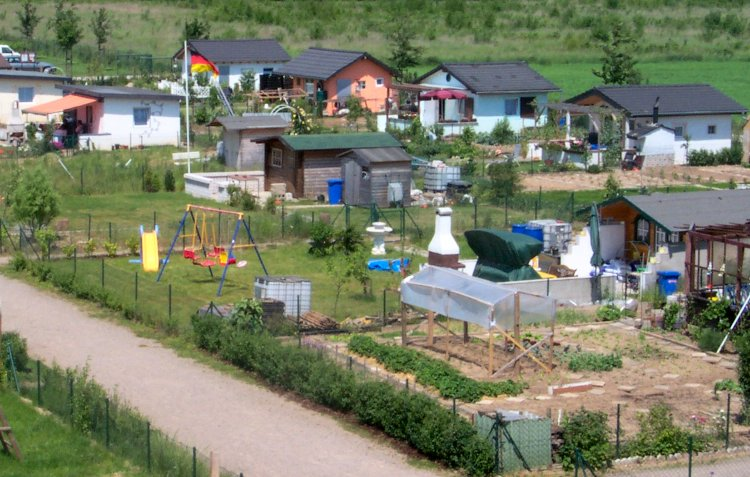
\includegraphics[width=0.5\textwidth]{images/Kleingarten.jpg}
	\caption[Bild von mehreren Parzellen einer Kleingartenanlage.]{
		Bild von mehreren Parzellen einer Kleingartenanlage.
		Zu sehen ist dabei die unterschiedliche Nutzung, die mittlere Parzelle wird als Spielplatz genutzt, während die vordere Parzelle für den Gemüseanbau genutzt wird.\footnotemark
	}
	\label{pic:kleingarten}
\end{figure}

\footnotetext{Bildquelle: Journey234, Public Domain, via Wikimedia Commons}

Bei einem Kleingarten, auch Schrebergarten genannt, handelt es sich um eine Parzelle in einer größeren Gartenanlage, wie sie beispielsweise in \cref{pic:kleingarten} zu sehen ist.
Kleingärten sind in Vereinen organisiert und die Mitglieder unterliegen der Kleingartensatzung des Vereins, woraus sich häufig spezielle Verpflichtungen und Einschränkungen ergeben, die bei Smart Gardening Lösungen berücksichtigt werden müssen.
Dabei kann es sich beispielsweise um Nutzungseinschränkungen für bestimmte Gerätetypen, Lärmschutz oder Verbot von Solaranlagen handeln.
Auch die Versorgung mit Strom und Wasser ist in verschiedenen Kleingartenanlagen unterschiedlich geregelt, wenn diese überhaupt vorhanden ist.
Es kann auch Verpflichtungen zur Art der Nutzung geben wie die Pflicht zum Anbau von Obst und Gemüse.
Daraus ergeben sich Anforderungen an die Flexibilität der Smart Gardening Lösungen.
Gleichzeitig muss beachtet werden, dass einige Smart Gardening Lösungen durch die Einschränkungen nicht oder nur eingeschränkt nutzbar sind.

Der Kleingarten wird auf verschiedene Arten und Weisen genutzt.
So nutzen einige Kleingärtner diesen zum Anbau von Obst und Gemüse, andere ihn zur Entspannung, was gut in \cref{pic:kleingarten} zu sehen ist.
Auch Imker sind in vielen Kleingärten vertreten, da der Imker von den vielen Pflanzen und die Kleingärtner von den Bienen profitieren.
Da diese Gartenart räumlich vom Wohnort getrennt ist, kann es sein, dass es immer wieder zu längeren Abwesenheiten des Hobbygärtners kommt.
Daher ist es von Vorteil, wenn die Smart Gardening Lösung auch ohne ständige Anwesenheit funktioniert.

\subsubsection{Hintergarten}
\begin{figure}[!htb]
	\centering
	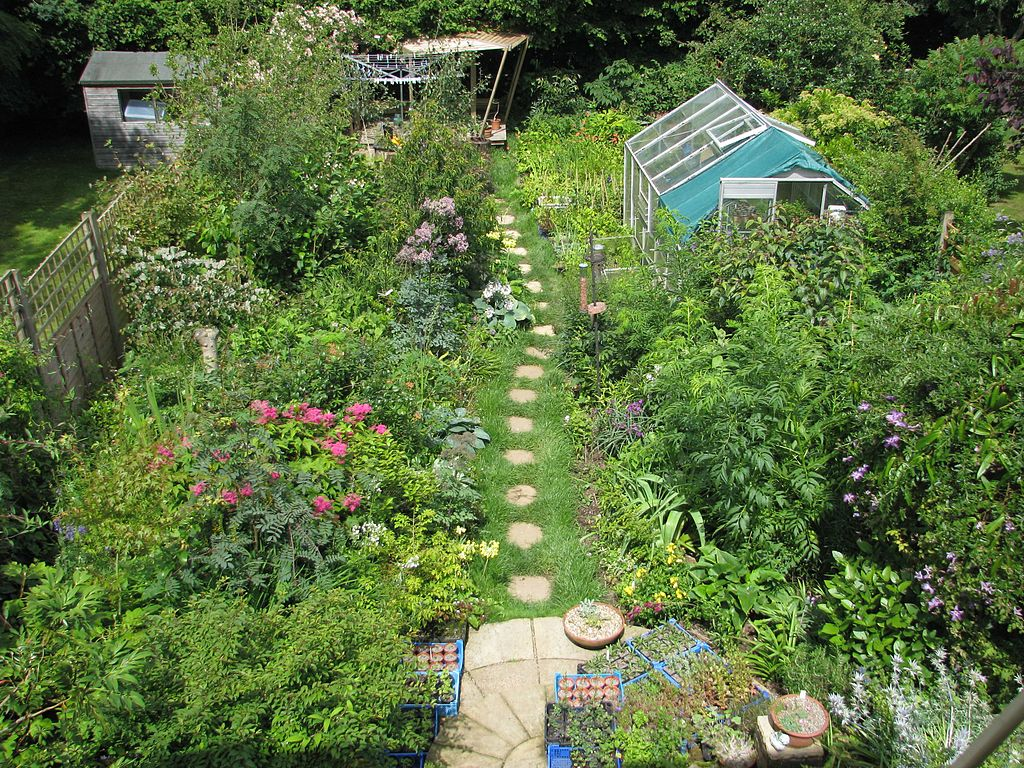
\includegraphics[width=0.5\textwidth]{images/Hintergarten.jpg}
	\caption[Bild eines kleinen, dicht bewachsenen Hintergartens.]{
		Bild eines kleinen, dicht bewachsenen Hintergartens.
		In diesem befinden sich viele verschiedene Pflanzen, ein Glasgewächshaus, eine Gartenhütte und eine Wäschespinne.
		Der Garten weist aufgrund des Bewuchses mit anderen Pflanzen keine größere Rasenfläche auf.\footnotemark
	}
	\label{pic:hintergarten}
\end{figure}

Viele Reihenhäuser und Einfamilienhäuser weisen einen Hintergarten auf.
Dieser ist meist eingezäunt und kann ansonsten viele verschiedene Formen und Größen aufweisen, wie in \cref{pic:hintergarten} zu sehen.
Dabei ist dieser häufig größer als ein Vorgarten, weshalb hier umfangreichere Smart Gardening Lösungen umgesetzt werden können.
Gleichzeitig sind große Teile des Gartens weiter vom Haus entfernt, was in dem Beispielbild gut zu sehen ist.

Normalerweise hat ein solcher Garten einen Rasen, welcher regelmäßig gemäht werden muss, wofür sich Mähroboter anbieten.
Auch verschiedene Beete und Bäume sind hier häufig zu finden, was in \cref{pic:hintergarten} gut zu sehen ist.
Je nach Größe des Gartens erfordern diese viel Pflege und Aufmerksamkeit, weshalb Smart Gardening Lösungen hier eine große Hilfe sein können.
Insbesondere die Bewässerung muss in Trockenperioden regelmäßig erfolgen, wofür sich automatische Bewässerungssysteme anbieten.
Hierbei ist es wichtig, dass die Sensoren und Aktuatoren auch in den hinteren Teilen des Gartens zuverlässig funktionieren.
Weiterhin weisen viele Hintergärten ein Gartenhaus zur Lagerung von unter anderem Werkzeug auf und einige haben auch ein Gewächshaus für den Anbau von Pflanzen, wie in \cref{pic:hintergarten} zu sehen.

\footnotetext{Bildquelle: peganum, \href{https://creativecommons.org/licenses/by-sa/2.0}{CC BY-SA 2.0}, via Wikimedia Commons}

Eine besondere Art des Hintergartens ist der große Garten, wobei die Abgrenzung in der Realität fließend ist.
Hier wird analog zu~\cite{grosserGarten} ein Garten als großer Garten bezeichnet, wenn er größer als 1.000 Quadratmeter ist.
Große Gärten weisen besondere Herausforderungen auf.
Um einen solchen Garten vollständig mit Smart Gardening ausstatten zu können, muss eine solche Lösung skalierbar sein.
Außerdem hat ein großer Garten potenziell mehr verschiedene Elemente, die mit unterschiedlichen Sensoren eingebunden werden wollen.
Welche Smart Gardening Lösungen für die jeweiligen Elemente geeignet sind, wird in den entsprechenden Abschnitten erläutert.

\subsubsection{Landschaftsgarten}
\begin{figure}[!htb]
	\centering
	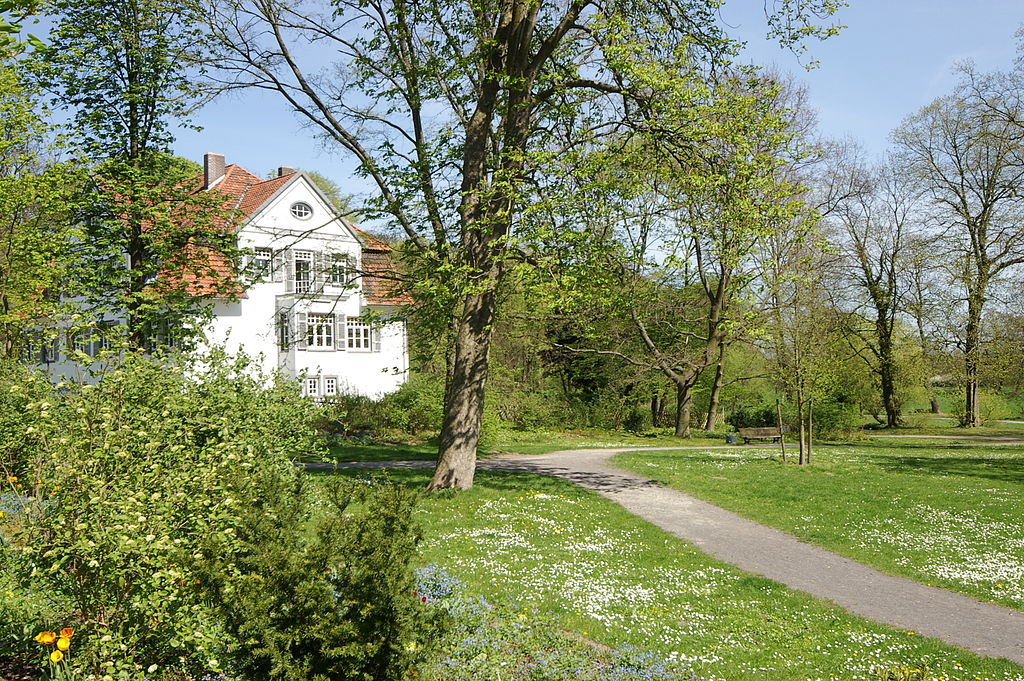
\includegraphics[width=0.5\textwidth]{images/Landschaftsgarten.jpg}
	\caption[Bild eines Landschaftsgartens mit einem Weg, Bäumen und Büschen.]{
		Bild eines Landschaftsgartens mit einem Weg und mehreren Bäumen und Büschen.\footnotemark
	}
	\label{pic:landschaftsgarten}
\end{figure}

Landschaftsgärten sind größere Gärten, die normalerweise nicht einem Haushalt zugeordnet sind, wie in Parks.
Ein Beispiel dafür ist in \cref{pic:landschaftsgarten} zu sehen, wobei dieser Landschaftsgarten von einem Weg durchzogen ist.
Sie dienen der Verschönerung und Erholung, sind meist der Öffentlichkeit zugänglich und werden häufig von professionellen Gärtnern gepflegt.
Daher sind hier Smart Gardening Lösungen sinnvoll, die den Gärtner in seiner Arbeit unterstützen, ihm also Arbeit abnehmen, ihm Kosten oder Zeit sparen oder die Qualität der Arbeit verbessern.
Aufgrund der öffentlichen Nutzung besteht eine erhöhte Gefahr von Diebstahl oder Vandalismus, weshalb die Smart Gardening Lösungen robust und sicher sein müssen.
Gleichzeitig sollten sie sich unauffällig in die Umgebung integrieren lassen, um das Erscheinungsbild nicht zu stören und gleichzeitig diese Gefahr zu minimieren.
Da Landschaftsgärten meistens größer sind als andere Gärten, müssen die Sensoren und Aktuatoren flächenmäßig skalierbar eingesetzt werden können.

\footnotetext{Bildquelle: Ingo Rickmann Ricki, \href{https://creativecommons.org/licenses/by-sa/2.5}{CC BY-SA 2.5}, via Wikimedia Commons}

\subsubsection{Landwirtschaft}
Die Landwirtschaft ist ein weiteres Umfeld, in dem Smart Gardening eingesetzt werden kann.
Aufgrund der Diversität dieses Umfelds und dem Fokus auf vor allem Hobbygärtner und nachrangig professionelle Gärtner wird hier nur ein kurzer Überblick gegeben.
Des Weiteren werden die Anforderungen an Smart Gardening zwar theoretisch genannt, aber nicht in die Anforderungsmenge aufgenommen.
Landwirtschaft setzt sich zusammen aus dem wirtschaftlichen Betrieb von Ackerbau und Viehwirtschaft.
Dabei gibt es verschiedene Formen von Landwirtschaft, die sich in der Größe und der Art der Bewirtschaftung unterscheiden.
Der Unterschied zur Gartenarbeit liegt in der Größe und der kommerziellen Nutzung.

\begin{figure}[!ht]
	\centering
	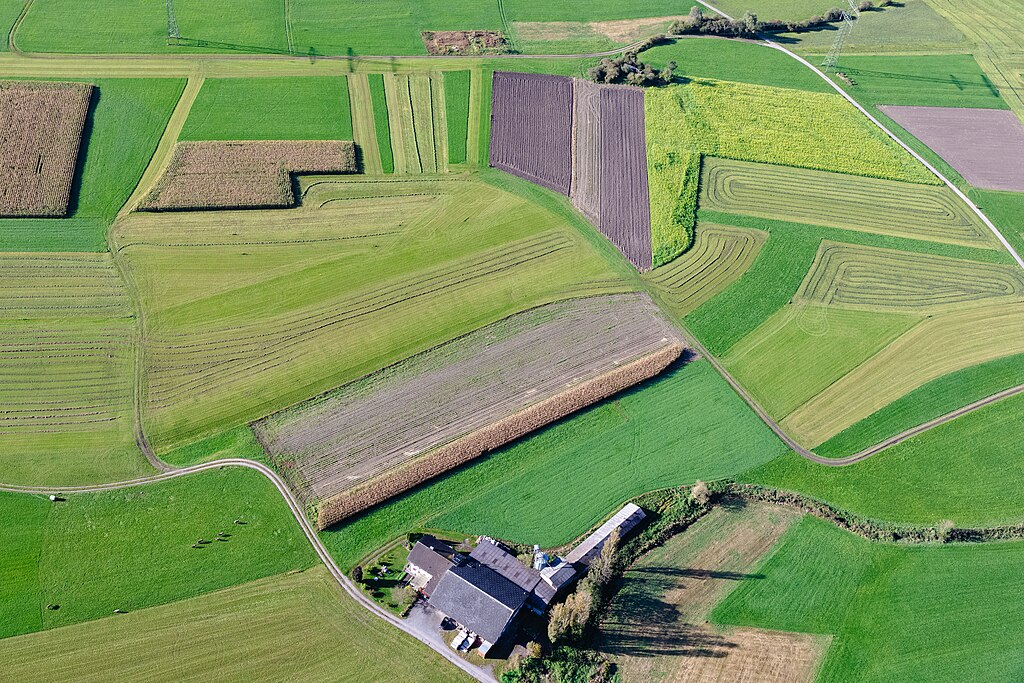
\includegraphics[width=0.5\textwidth]{images/Landwirtschaft.jpg}
	\caption[Bild einer kleinen landwirtschaftlich genutzten Fläche.]{
		Bild einer kleinen landwirtschaftlich genutzten Fläche.
		Außerdem ist ein Haus mit abgebildet.\footnotemark
	}
	\label{pic:landwirtschaft}
\end{figure}

In \cref{pic:landwirtschaft} ist eine kleine landwirtschaftlich genutzte Fläche zu sehen, die im Vergleich zu Gärten deutlich größer ist, gleichzeitig gibt es noch viel größere landwirtschaftliche Flächen.
Die Größe ist dabei eine Herausforderung für Smart Gardening, da die Sensoren und Aktuatoren entsprechend skalierbar sein müssen.
Wird etwa ein automatisches Bewässerungssystem eingesetzt, so muss die gesamte Fläche mit entsprechenden Feuchtigkeitssensoren und Bewässerungsdüsen ausgestattet werden.
Diese großflächige Ausstattung ist aufwendig und teuer, weshalb hier eine hohe Zuverlässigkeit und Effizienz gefordert ist.
Das Budget ist zwar größer als bei Gärtnern, aber die Fläche ist auch um ein Vielfaches größer.

\footnotetext{Bildquelle: Herbert Heim, \href{https://creativecommons.org/licenses/by-sa/4.0}{CC BY-SA 4.0}, via Wikimedia Commons}

\subsubsection{Zusammenfassung der Gartenarten}
Gerade wurde die Vielfalt der verschiedenen Gartenarten dargestellt.
Diese Liste ist nicht vollständig und kann es auch nicht sein, deckt aber die häufigsten Gärten ab.
Andere Gartenarten können als Unterarten oder Kombinationen dieser Gartenarten betrachtet werden.
So hat etwa ein japanischer Garten Elemente eines Landschaftsgartens und eines Vorgartens.

Dabei gibt es viele Gemeinsamkeiten, aber auch viele Unterschiede zwischen den verschiedenen Gartenarten.
Alle Gartenarten können in verschiedenen Arten von Smart Gardening Lösungen profitieren, wobei die Anforderungen an diese unterschiedlich sind.
Hierbei kann es sich beispielsweise um Arbeitserleichterungen, Kosteneinsparungen oder Ertragssteigerungen handeln.
Smart Gardening Lösungen benötigen für die meisten Gartenarten eine zusätzliche Strom- und Wasserversorgung, wobei die Internetverbindung in den meisten Fällen über WAN erfolgt.
In fast allen Gärten sind Schädlinge und andere Tiere ein Problem, weshalb eine Detektion und gegebenenfalls Verjagung notwendig ist.

\pagebreak

Gleichzeitig sind alle Gärten in unterschiedlicher Intensität den Elementen ausgesetzt, weshalb die Smart Gardening Lösungen robust sein müssen.
In den verschiedenen Gartenarten können nun unterschiedliche Gartenelemente vorkommen, auf die im nächsten Abschnitt eingegangen wird.


\subsection{Gartenelemente}
In diesem Abschnitt werden verschiedene Gartenelemente, die teilweise schon erwähnt wurden, erklärt und im Kontext von Smart Gardening analysiert.
Sie bringen eigene Eigenschaften und Anforderungen an Smart Gardening mit sich.
Dazu gehört, was diese Elemente ausmacht und was beachtet werden muss.
Zunächst werden gemeinsame Aspekte der verschiedenen Gartenelemente betrachtet.
Danach wird die folgende ausgewählte Teilmenge der Gartenelemente betrachtet, welche nach Ähnlichkeit sortiert ist: Rasen, Beet, Baum, Pflanzentopf, Gewächshaus, Regentonne, Brunnen, Gartenteich, Pool, Gartenhaus, Gehege / Stall, Bienenstock und Kompost.

Für die Analyse werde die Gartenelemente zunächst erklärt, danach werden sie voneinander abgegrenzt und ihre Besonderheiten herausgestellt.
Zum Schluss wird betrachtet, von welchen Messungen und Automatisierungen sie profitieren können.
Nach den einzelnen Gartenelementen folgt eine Zusammenfassung mit verschiedenen Tabellen zur Übersicht über die Gartenelemente.

\subsubsection{Gartenelementübergreifende Aspekte}
Zunächst werden gemeinsame Aspekte der verschiedenen Gartenelemente betrachtet, welche auf viele Gartenelemente zutreffen.
Fast alle Gartenelemente sind den Elementen ausgesetzt, wozu unter anderem Regen, Schnee, Wind, Sonne und Temperaturschwankungen zählen.
Ein automatisches Bewässerungssystem ist etwa der Luft- und Bodenfeuchtigkeit und Regen ausgesetzt, was aufgrund der Elektronik und Rost ein Problem darstellen kann.
Weiterhin ist ein Bewässerungssystem im Garten der Sonne ausgesetzt, was über längere Zeit zu Schäden führen kann.

Pflanzengartenelemente wie Rasen und Beete sind sich in vielen Aspekten besonders ähnlich.
Dazu gehört unter anderem die Bewässerung der Pflanzen, die notwendig für diese ist, wenn sie nicht durch Regen ausreichend versorgt werden.
Die Bewässerung kann durch ein automatisches Bewässerungssystem übernommen werden.
Die Koppelung dieser Bewässerung an Bodenfeuchtigkeitssensoren sowie an Wetterdaten kann die Bewässerung optimieren und so die Pflanzen besser versorgen.
Dabei kann die Bewässerung auch an die Art der Pflanzen angepasst werden, da verschiedene Pflanzen unterschiedliche Wassermengen benötigen.
Frost kann solche Bewässerungssysteme potenziell beschädigen, weshalb eine Temperaturmessung in Kombination mit Wetterdaten helfen kann, Frost zu erkennen und das Bewässerungssystem abzuschalten.
Gleichzeitig kann der Nutzer über diese Gefahr informiert werden, damit er eventuelle weitere Gegenmaßnahmen einleiten kann.
Als Wasserquelle für ein solches Bewässerungssystem können ein Außenwasseranschluss, ein Brunnen oder eine Wassertonne dienen.

Ein weiterer Aspekt ist die Düngung der Pflanzen, welche regelmäßig erfolgen muss, um die Pflanzen optimal zu versorgen.
Hierbei ist zu beachten, dass falsches Düngen zum Einen die Umwelt belasten und zum Anderen die Pflanzen schädigen kann~\cite{RasenDuenger}.
Durch Messungen kann etwa der Stickstoffgehalt und Phosphorgehalt im Boden gemessen werden, woraus abgeleitet werden kann, wann und wie viel Dünger benötigt wird.
Hierbei sollte bei der Auswahl der überwachten Stoffe im Boden darauf geachtet werden, dass diese relevant für die Pflanzen sind.
Ein intelligentes System kann basierend auf diesen Daten den Nutzer informieren, wann und wie viel gedüngt werden soll.
Auch der pH-Wert des Bodens ist wichtig, weshalb der Nutzer bei einer größeren Abweichung vom Idealwert informiert werden kann.
So kann er rechtzeitig Gegenmaßnahmen einleiten, wie das Kalken des Bodens.

\subsubsection{Gartenelement Rasen}
\begin{figure}[!htb]
	\centering
	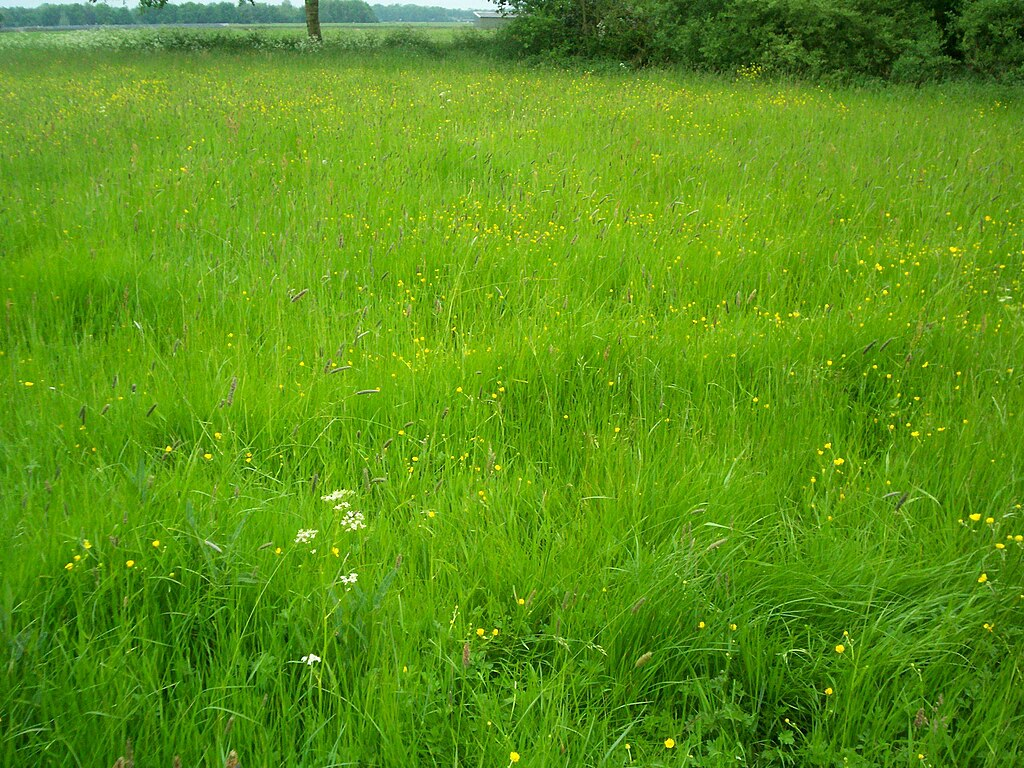
\includegraphics[width=0.5\textwidth]{images/Rasen.jpg}
	\caption[Bild eines wild wachsenden Rasens, der seit Längerem nicht gemäht wurde.]{
		Ein wild wachsender Rasen, der seit Längerem nicht gemäht wurde.
		Auch Blumen wachsen auf der Rasenfläche.\footnotemark
	}
	\label{pic:rasen}
\end{figure}

\footnotetext{Bildquelle: Natubico, \href{https://creativecommons.org/licenses/by-sa/3.0}{CC BY-SA 3.0}, via Wikimedia Commons}

Ein Rasen ist eine weitverbreitete Vegetationsdecke aus verschiedenen Gräsern, wie sie in \cref{pic:rasen} zu sehen ist.
Sie wird häufig in Gärten und Parks angelegt und muss regelmäßig gepflegt werden.
Zu dieser Pflege gehört das Mähen, das Bewässern und das Düngen.
Dabei gibt es verschiedene Möglichkeiten den Rasen zu mähen, wie mit Tieren wie Ziegen, verschiedenen Arten von Rasenmähern und neuerdings auch mit Mährobotern.
Das manuelle Mähen mit einem Rasenmäher ist zeitaufwendig und anstrengend, weshalb automatische Mähroboter eine gute Alternative darstellen.
Diese können auf verschiedene Arten gesteuert werden, wozu Regeln, Apps und verschiedene Schnittstellen gehören.
Eine solche Regel kann einfach zeitbasiert, aber auch komplex abhängig von Sensorwerten sein.
Durch komplexere Regeln kann das Mähen an die Situation angepasst werden.
Rasen wächst bei unterschiedlichen Temperaturen unterschiedlich schnell und ist bei hohen Temperaturen empfindlicher, weshalb die Mähfrequenz angepasst werden sollte.
Dabei können sowohl Wetterdaten als auch Sensoren für die Temperatur helfen.
Die Bewässerung kann von automatischen Bewässerungssystemen übernommen werden, wie in den gartenelementübergreifenden Aspekten beschrieben.
Auch die Düngung des Rasens kann, wie in den gartenelementübergreifenden Aspekten beschrieben, automatisiert unterstützt werden.

\subsubsection{Gartenelement Beet}
\begin{figure}[!htb]
	\centering
	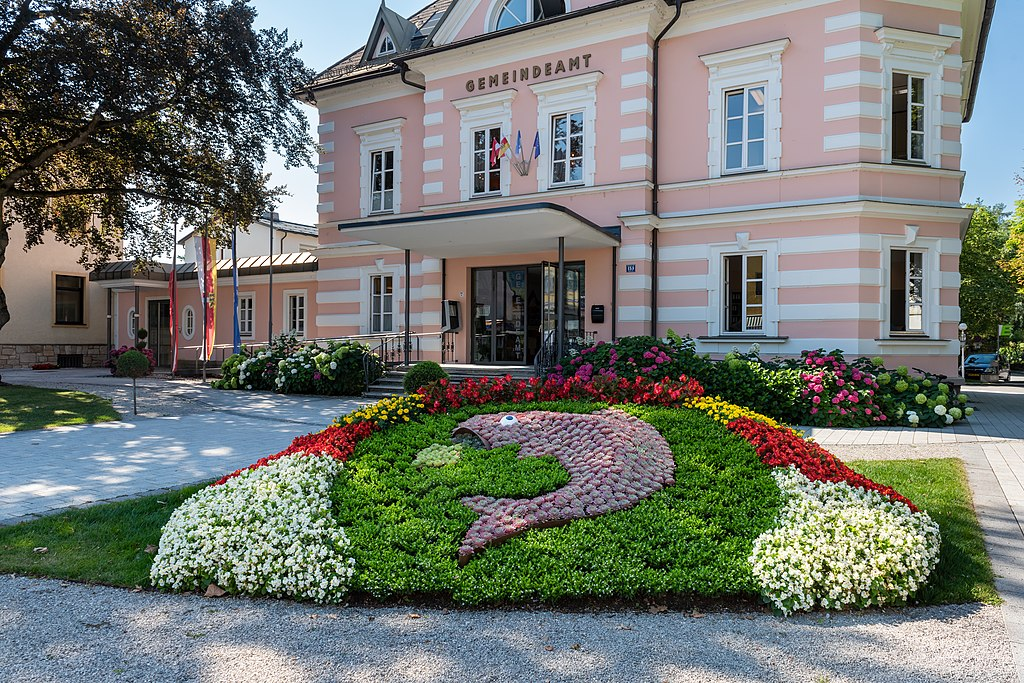
\includegraphics[width=0.49\textwidth]{images/Blumenbeet.jpg}
	\includegraphics[width=0.49\textwidth]{images/Gemüsebeet.jpg}
	\caption[Bilder von verschiedenen Beeten.]{Zwei Bilder von verschiedenen Beeten.
		Auf dem linken Bild ist ein Hügel-Blumenbeet zu sehen, welches mit den Blumen ein Muster bildet.
		Auf der rechten Seite ist Boden-Gemüsebeet zu sehen, in welchem in langen Reihen verschiedene Gemüsesorten wachsen.\footnotemark
	}
	\label{pic:beet}
\end{figure}

\footnotetext{Bildquellen:\\
	Links: Johann Jaritz, \href{https://creativecommons.org/licenses/by-sa/4.0}{CC BY-SA 4.0}, via Wikimedia Commons\\
	Rechts: Burkhard Mücke, \href{https://creativecommons.org/licenses/by-sa/4.0}{CC BY-SA 4.0}, via Wikimedia Commons
}

Ein Beet ist ein Bereich, in dem Pflanzen angebaut werden.
Es gibt verschiedene Arten und Formen von Beeten, wie in \cref{pic:beet} zu sehen.
Bei der Unterscheidung von Beeten kann nach der Art der Pflanzen und nach der Form unterschieden werden, wobei beliebige Kombinationen möglich sind.
So ist in \cref{pic:beet} links ein Blumenbeet als Hügelbett zu sehen, während rechts ein Gemüsebeet als Bodenbeet zu sehen ist.

Bei der Art der Pflanzen sind unter anderem Blumenbeete, Obst- und Gemüsebeete, Kräuterbeete und Staudenbeete möglich.
Je nach Art der Pflanzen können sich die Anforderungen an Smart Gardening geringfügig unterscheiden.
So dient ein Blumenbeet meist der Verschönerung des Gartens, weshalb hier die Optik eine größere Rolle spielt.
Ein Gemüsebeet hingegen dient der Selbstversorgung, weshalb hier die Menge und Qualität der Ernte eine größere Rolle spielen.
Gleichzeitig ähneln sich die Anforderungen an die Pflege, insbesondere bei der Bewässerung, dem Düngen und dem Entfernen von Unkraut.
Daher gelten unabhängig von der Art und Bepflanzung die gartenelementübergreifenden Aspekte für die automatische Bewässerung und Düngung.
Weiterhin benötigen verschiedene Pflanzen unterschiedliche Licht- und Temperaturbedingungen~\cite*{RosenTemperatur}.
Durch die Nutzung von Wetterdaten in Kombination mit Temperaturmessungen kann der Nutzer informiert werden, wenn die Bedingungen nicht optimal sind und es zu warm oder zu kalt ist oder wird.
Die Blüten und Früchte von Pflanzen können beispielsweise bei Frost Schaden nehmen, weshalb eine zeitige Reaktion des Nutzers notwendig ist.
In solchen Fällen kann der Nutzer handeln, um die Bedingungen zu verbessern, indem er die Pflanzen beispielsweise abdeckt, um die Temperatur zu halten und Frost zu vermeiden.

Für die Form gibt es verschiedene Möglichkeiten wie Hügelbeete, Bodenbeete und Hochbeete, wobei diese Einfluss auf beispielsweise die Bewässerung haben
Hochbeete benötigen bei gleicher Bepflanzung eine andere Bewässerung als Bodenbeete, da das Wasser im Hochbeet schneller abläuft.
Gleichzeitig sorgt die Erhöhung auch dafür, dass für das Bewässerungssystem Gravitation nicht mehr genutzt werden kann und somit auf eine andere Art Wasserdruck erzeugt werden muss.
Daher ist es wichtig, dass Smart Gardening Lösungen an die Form des Beetes angepasst werden können.
Auch Aspekte wie die Düngung können von der Form des Beetes abhängen, da Hügelbeete wie in \cref{pic:beet} häufig mit Kompost gebaut werden und somit der Düngebedarf unterschiedlich ist.

\subsubsection{Gartenelement Baum}
\begin{figure}[!htb]
	\centering
	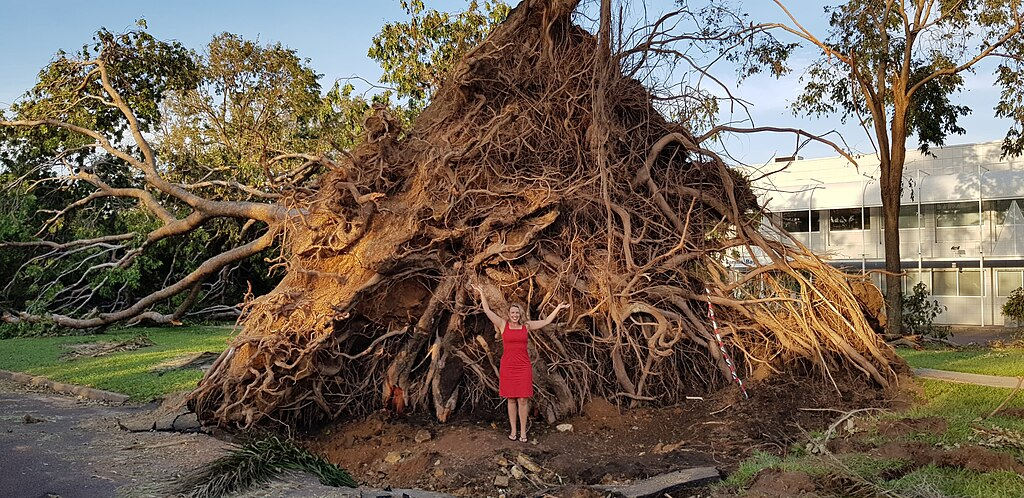
\includegraphics[width=0.7\textwidth]{images/Wurzeln.jpg}
	\caption[Bild eines umgekippten Baumes.]{
		Bild eines umgekippten Baumes.
		Der Baum liegt entwurzelt auf der Seite, wodurch das tiefe Wurzelwerk sichtbar wird.\footnotemark
	}
	\label{pic:baum}
\end{figure}

\footnotetext{Bildquelle: Kclovelock, \href{https://creativecommons.org/licenses/by-sa/4.0}{CC BY-SA 4.0}, via Wikimedia Commons}

Bäume sind Holzgewächse, die in Gärten und Wäldern vorkommen, hunderte Jahre alt und über zehn Meter groß werden können.
Auch Bäume benötigen Pflege, um gesund zu bleiben.
Insbesondere junge Bäume müssen regelmäßig gegossen werden, aber auch ältere Bäume können von einer Bewässerung in Trockenperioden profitieren.
Die automatische Bewässerung, wie in den gartenelementübergreifenden Aspekten beschrieben, kann hier nicht eingesetzt werden.
Bäume haben ein tiefes Wurzelsystem wie in \cref{pic:baum} zu sehen, weshalb die Messung der Bodenfeuchtigkeit in der Nähe des Baumes nicht aussagekräftig ist und somit übermäßig gegossen werden kann.
Daher ist hier ein größerer Fokus auf die Wetterdaten wichtig, wobei diese mit Informationen über das Alter und die Art des Baumes kombiniert werden können.
Daraus kann abgeleitet werden, wie viel und wie oft der Baum gegossen werden muss.
Außerdem benötigen Bäume aufgrund ihrer Größe im Vergleich zu anderen Pflanzen mehr Wasser, weshalb dies bei der Wahl der Wasserquelle berücksichtigt werden muss.

\subsubsection{Gartenelement Pflanzentopf}
\begin{figure}[!htb]
	\centering
	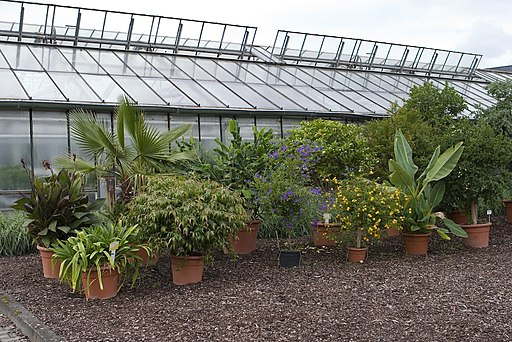
\includegraphics[width=0.5\textwidth]{images/Topf.jpg}
	\caption[Bild einer Reihe von Pflanzentöpfen.]{
		Bild einer Reihe von Pflanzentöpfen.
		Die Töpfe sind verschieden groß und mit unterschiedlichen Pflanzen bepflanzt.\footnotemark
	}
	\label{pic:topf}
\end{figure}

\footnotetext{Bildquelle: Martin Bahmann, \href{https://creativecommons.org/licenses/by-sa/3.0}{CC BY-SA 3.0}, via Wikimedia Commons}

Ein Pflanzentopf ist ein Behälter, der zum Anpflanzen von Pflanzen verwendet wird.
Er ist in verschiedenen Größen und Materialien erhältlich wie in \cref{pic:topf} und kann im Innen- oder Außenbereich verwendet werden.
Töpfe werden für die Kultivierung von Pflanzen auf Terrassen, Balkonen oder in Gärten eingesetzt.
Smart Gardening kann eingesetzt werden, um die Pflege von Pflanzen in Töpfen zu erleichtern.
Für die Bewässerung und Düngung gelten die gartenelementübergreifenden Aspekte.
Weiterhin können die Pflanzen von Licht- und Temperaturmessungen profitieren, da verschiedene Pflanzen unterschiedliche Licht- und Temperaturbedingungen benötigen.
Durch die Messung dieser Werte kann der Nutzer informiert werden, wenn die Bedingungen nicht optimal sind.
Je nach Position des Pflanzentopfes können auch Wetterdaten relevant sein, um etwa eine Warnung auszugeben, wenn Sturm oder Hagel droht.
In so einem Fall können die Pflanzen geschützt werden.
Diese Smart Gardening Überlegungen für Töpfe können auch auf Balkonkästen und Blumenkästen übertragen werden.

\subsubsection{Gartenelement Gewächshaus}\label{sec:gartenlement-gewächshaus}
Zuvor wurde bereits das Gewächshaus als Gartenart betrachtet.
Nun wird das Gewächshaus als Gartenelement betrachtet, wobei der Fokus auf Glasgewächshäusern liegt wie links in \cref{pic:gewächshaus}.
Als kontrollierte Umgebung kann das Gewächshaus von diverser Sensorik und Aktuatorik profitieren.
Pflanzen haben Temperaturanforderungen für ein gutes Wachstum, weshalb die Temperatur ein wichtiger Faktor ist.
Durch regelmäßige Temperaturmessungen kann überwacht werden, ob die Temperatur den optimalen Bereich verlässt.
Geschieht dies, so kann beispielsweise durch Heizen oder Lüften automatisiert gegengesteuert werden.
Die Luftfeuchtigkeit ist ein weiterer wichtiger Faktor.
Auch hier können Messungen und automatisierte Gegenmaßnahmen eingesetzt werden, wie mit Luftbefeuchtern, Luftentfeuchtern und Lüften.
Da Pflanzen Licht zum Wachsen benötigen, ist die Messung der Lichtintensität wichtig.
Diese Messung kann genutzt werden, um automatisiert die Beleuchtung zu steuern.
Pflanzen profitieren auch von einem erhöhten CO$_2$-Gehalt in der Luft, weshalb es von Vorteil ist diesen zu messen und automatisiert zu steuern~\cite{PflanzenCO2}.
Für die Bewässerung und Düngung gelten die gartenelementübergreifenden Aspekte.
In all diese Maßnahmen können Wetterdaten einfließen.

\subsubsection{Gartenelement Regentonne}
\begin{figure}[!htb]
	\centering
	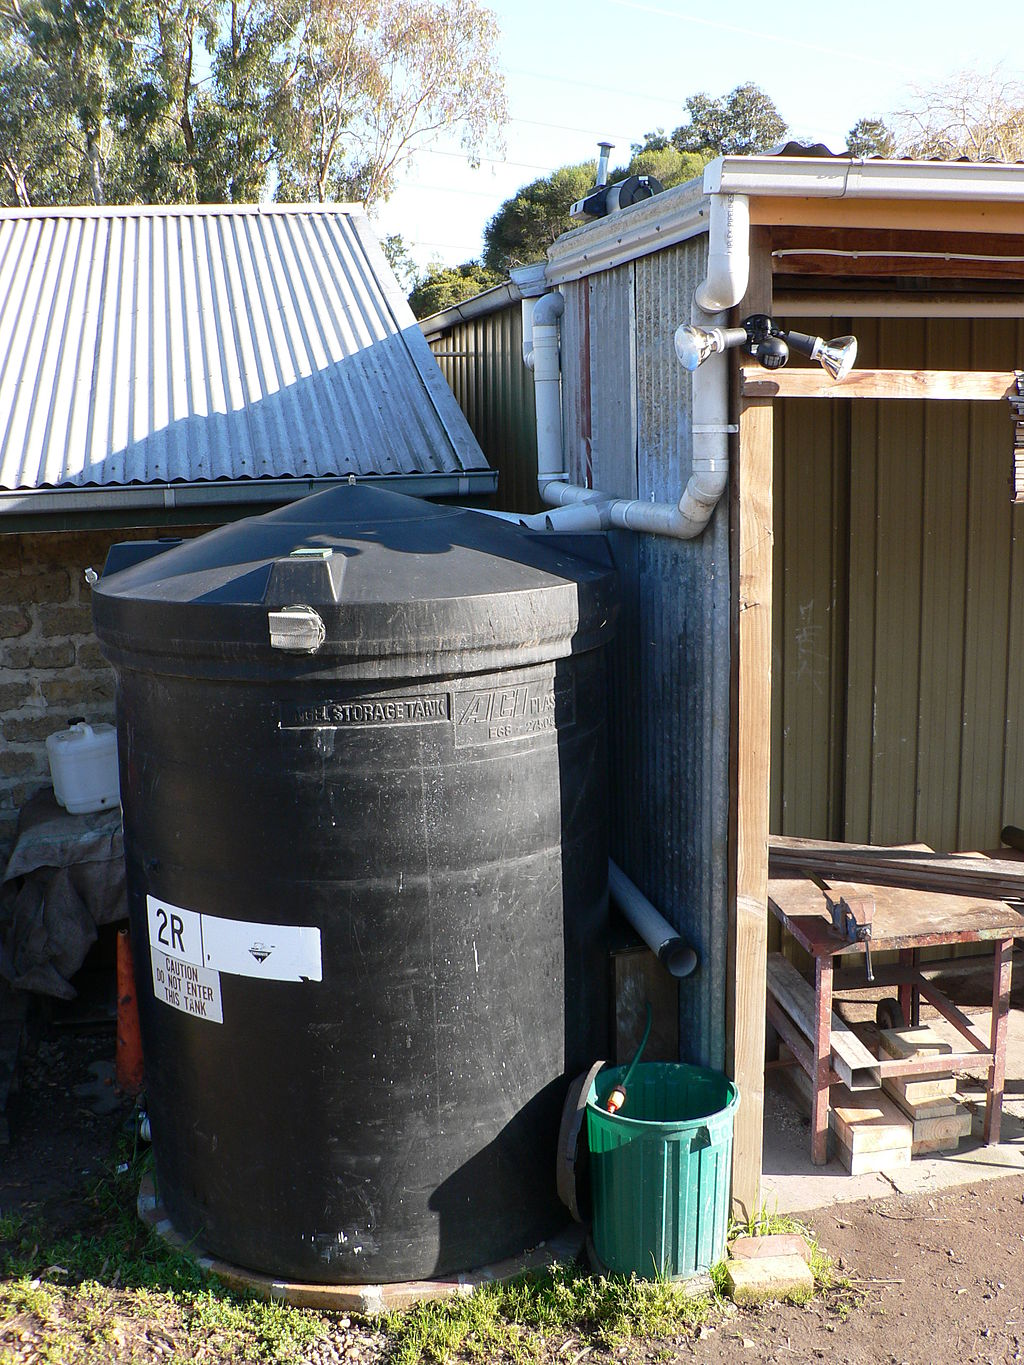
\includegraphics[height=0.4\textheight]{images/Regentonne.jpg}
	\caption[Bild einer Regentonne, die am Deckel einen Zulauf hat.]{
		Bild einer Regentonne, die am Deckel einen Zulauf hat, der von Dachrinnen gefüllt werden kann.\footnotemark
	}
	\label{pic:regentonne}
\end{figure}

\footnotetext{Bildquelle: Pengo, \href{https://creativecommons.org/licenses/by-sa/3.0}{CC BY-SA 3.0}, via Wikimedia Commons}

Eine Regentonne ist ein Behälter, der Regenwasser sammelt.
Wie in \cref{pic:regentonne} zu sehen, wird das Regenwasser zunächst in Dachrinnen gesammelt und dann über Leitungen in eine Regentonne oder einen anderen Behälter geleitet.
Dadurch können große Mengen an Wasser gesammelt werden, insbesondere bei großen Dachflächen und langem und starkem Regen.
Dieses gesammelte Regenwasser kann dann zur Bewässerung von Pflanzen im Garten verwendet werden, wodurch Wasser und Geld gespart werden kann.
Außerdem ist Regenwasser je nach Region besser für Pflanzen als Leitungswasser, insbesondere wenn das Leitungswasser gechlort ist~\cite{PflanzenChlor}.
Regentonnen können als Wasserquelle für automatische Bewässerungssysteme genutzt werden.
Daher ist es wichtig, den Füllstand der Tonne zu messen, was mittels Pegelmessgeräten möglich ist.
Durch die Messung des Füllstands kann der Nutzer informiert werden, wann die Tonne leer oder voll ist.
In Kombination mit Wetterdaten und Daten eventuell angeschlossener automatischer Bewässerungssysteme kann eine Füllstandprognose erzeugt werden.
Außerdem sind Regentonnen anfällig für Frost, da sich zum einen Wasser beim Gefrieren ausdehnt und zum anderen einige Materialien spröde werden können.
Daher kann eine Temperaturmessung helfen, Frost zu erkennen und die Tonne zu schützen, indem etwa das Wasser abgelassen wird.

\subsubsection{Gartenelement Brunnen}
\begin{figure}[!htb]
	\centering
	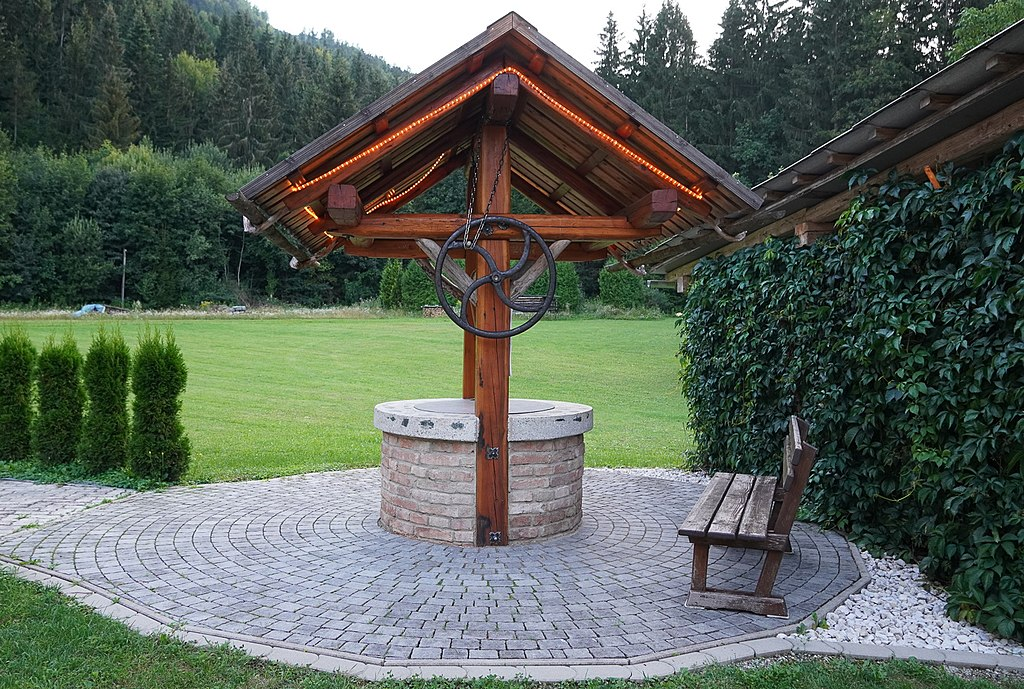
\includegraphics[height=0.32\textheight]{images/Ziehbrunnen.jpg}
	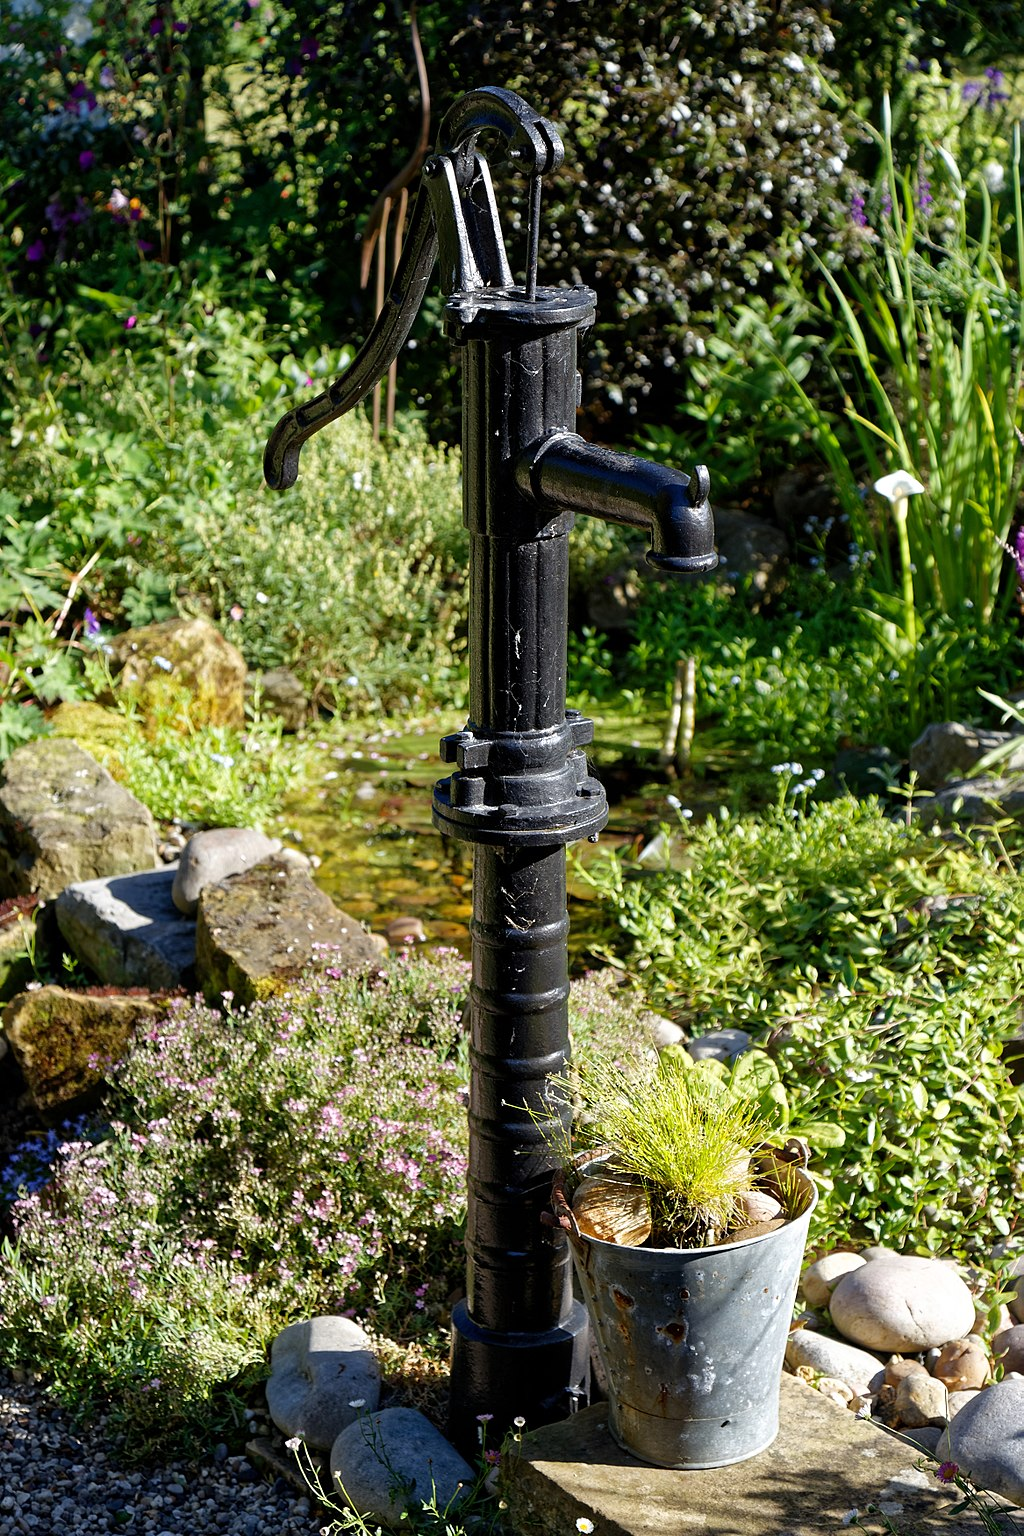
\includegraphics[height=0.32\textheight]{images/Handpumpe.jpg}
	\caption[Bilder von verschiedenen Arten von Brunnen.]{
		Zwei Bilder von verschiedenen Arten von Brunnen.
		Auf der linken Seite ist ein Ziehbrunnen, der heutzutage primär als dekoratives Element verwendet wird.
		Auf der rechten Seite ist ein Brunnen mit Handpumpe, wobei es ähnliche Brunnen auch mit motorisierter Pumpe gibt.
		Dieser Brunnen dient primär als Wasserquelle.\footnotemark
	}
	\label{pic:brunnen}
\end{figure}
\footnotetext{Bildquellen:\\
	Naturpuur, \href{https://creativecommons.org/licenses/by-sa/4.0}{CC BY-SA 4.0}, via Wikimedia Commons\\
	Acabashi, \href{https://creativecommons.org/licenses/by-sa/4.0}{CC BY-SA 4.0}, via Wikimedia Commons
}

Ein Brunnen ist eine Struktur, die Wasser aus einer unterirdischen Quelle verfügbar macht.
Brunnen werden in Gärten oft als dekoratives Element verwendet, können aber auch als Wasserquelle im Garten dienen.
Dabei gibt es verschiedene Arten von Brunnen, wie Ziehbrunnen und Brunnen mit einer Pumpe, wie in \cref{pic:brunnen} zu sehen.
Heutzutage werden Ziehbrunnen primär als dekoratives Element verwendet, während Brunnen mit einer Pumpe als Wasserquelle dienen.
So kann ein Brunnen mit Pumpe in ein automatisches Bewässerungssystem eingebunden werden, wobei auch die gepumpte Wassermenge gemessen werden kann.
Abgesehen davon ist ein Brunnen auch für Frost anfällig, weshalb eine Temperaturmessung helfen kann, Frost zu erkennen und den Brunnen zu schützen.
Auch Wetterdaten können hierfür sinnvoll eingesetzt werden.

\subsubsection{Gartenelement Gartenteich}
\begin{figure}[!htb]
	\centering
	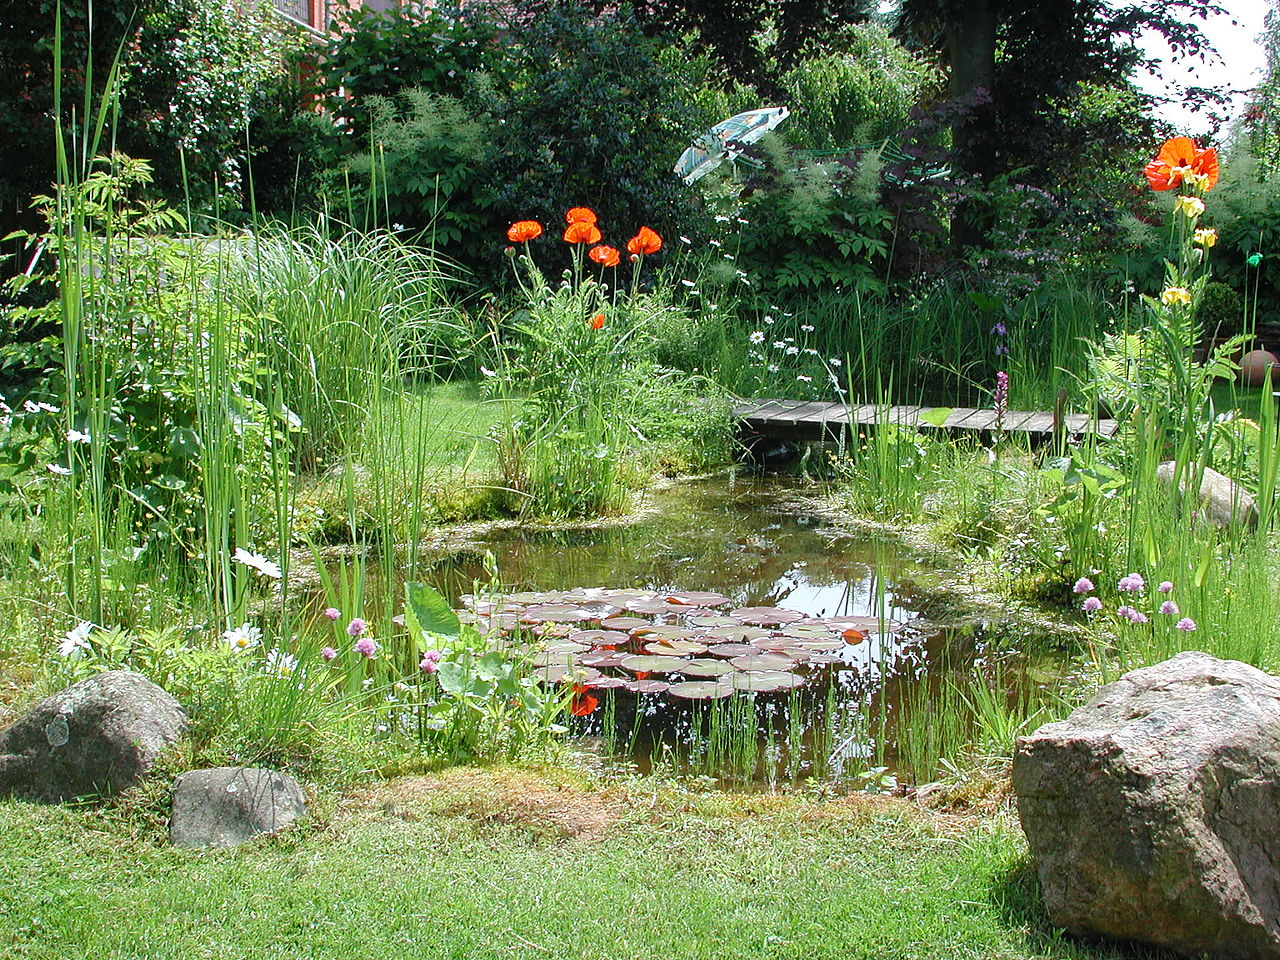
\includegraphics[width=0.5\textwidth]{images/Gartenteich.jpg}
	\caption[Bild eines Gartenteichs.]{
		Bild eines Gartenteichs.
		Der Teich hat eine mittlere Größe und ist mit verschiedenen Pflanzen sowohl am Ufer als auch im Wasser selbst bewachsen.
		Das Wasser ist aufgrund der Menge an Algen grün.\footnotemark
	}
	\label{pic:gartenteich}
\end{figure}

\footnotetext{Bildquelle: Matthias Wilke, \href{https://creativecommons.org/licenses/by-sa/3.0}{CC BY-SA 3.0}, via Wikimedia Commons}

Ein Gartenteich ist ein kleines Gewässer im Garten, welches natürlich oder künstlich angelegt sein kann und in verschiedenen Varianten existiert.
Wie in \cref{pic:gartenteich} zu sehen, kann er beispielsweise von Fischen, Fröschen, Schnecken oder anderen Tieren bewohnt sein, gleichzeitig können auch verschiedene Pflanzenarten im Teich wachsen.
Zur Kontrolle des Wasserspiegels können Pumpen eingesetzt werden.
Ein solcher Teich benötigt regelmäßige Pflege, wie das Entfernen von Algen, das Reinigen des Wassers und das Füttern der Tiere.
Dazu gehört auch die regelmäßige Prüfung der Wasserqualität, um die Gesundheit der Bewohner zu gewährleisten.
Die Wasserqualität setzt sich dabei aus verschiedenen Werten wie der Wasserhärte, dem pH-Wert, dem Sauerstoffgehalt, Nitrit, Nitrat, Ammonium und Ammoniak.
Außerdem fördert ein Überschuss an Nährstoffen das Algenwachstum, was die Wasserqualität verschlechtert und für viele Menschen weniger gut aussieht, wie in \cref{pic:gartenteich} zu sehen.
Wichtig zu beachten sind Wechselwirkungen zwischen den Werten des Teichs, wie zwischen Temperatur und Sauerstoffkonzentration.
So kann Wasser bei niedrigen Temperaturen mehr Sauerstoff lösen.
Auch wichtig ist die Messung des Wasserspiegels, da zu niedriger Wasserspiegel die Pumpe beschädigen und den Tieren und Pflanzen schaden kann~\cite{TeichFische}.
Auf Basis dieser Messung kann der Nutzer benachrichtigt werden, um den Wasserspiegel zu erhöhen.
Auch eine automatische Bewässerung kann hier eingesetzt werden.
Die Fütterung der Tiere kann durch regelbasierte Fütterungssysteme erfolgen.
Diese können die Messwerte der Wasserqualität nutzen, um zu entscheiden, ob und wie viel gefüttert werden soll.
Die Messwerte der Wasserqualität können auch genutzt werden, um automatische Gegenmaßnahmen zu starten.
Dazu gehören unter anderem das Einschalten einer Pumpe oder das Hinzufügen von Chemikalien.

\subsubsection{Gartenelement Pool}
\begin{figure}[!htb]
	\centering
	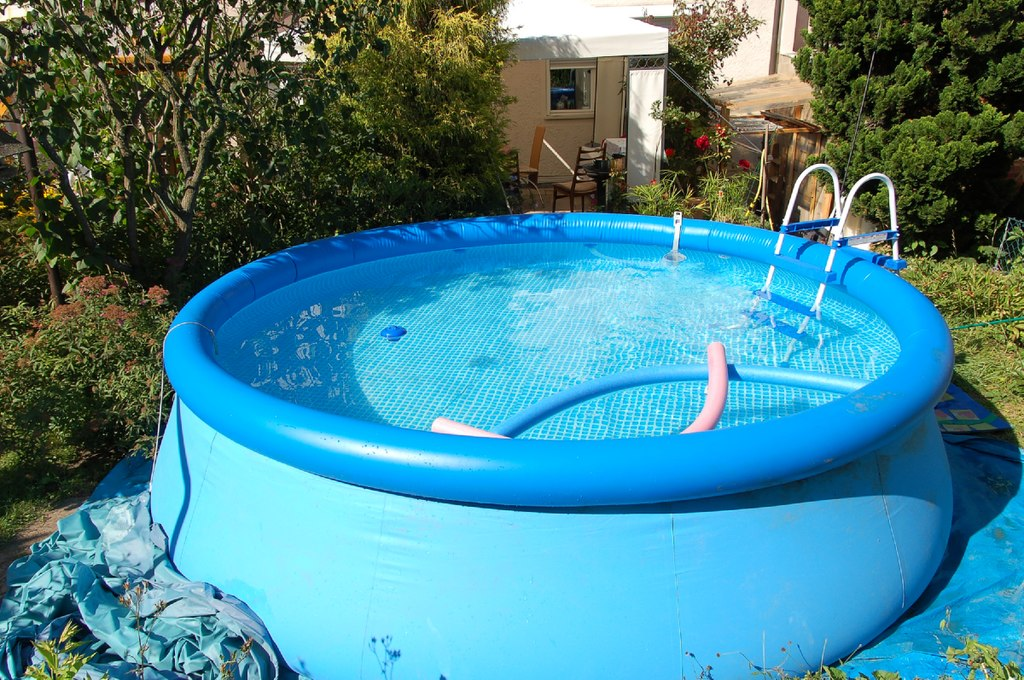
\includegraphics[width=0.5\textwidth]{images/Pool.jpg}
	\caption[Bild eines aufblasbaren Pools in einem Hintergarten.]{
		Bild eines aufblasbaren Pools in einem Hintergarten.
		Der Pool besitzt eine Pumpe zur Reinigung des Wassers und eine Leiter zum Ein- und Aussteigen.\footnotemark
	}
	\label{pic:pool}
\end{figure}

\footnotetext{Bildquelle: Ra Boe, \href{https://creativecommons.org/licenses/by-sa/3.0}{CC BY-SA 3.0}, via Wikimedia Commons}

Ein Pool ist ein künstlich angelegtes Wasserbecken, das zum Schwimmen, Erholen und Spaß haben genutzt wird.
Pools können verschiedene Formen und Größen haben, können im Boden eingelassen oder aufgestellt sein.
Pools benötigen regelmäßige Pflege, um die Wasserqualität zu erhalten.
Wie in \cref{pic:pool} zu sehen, werden dafür selbst in aufblasbaren Pools Pumpen und Filter eingesetzt, um das Wasser zu reinigen.
Diese Filter können aber nicht alle Schadstoffe entfernen, weshalb die Wasserqualität auch durch den Nutzer überwacht werden muss.
Eine gute Wasserqualität ist wichtig für die Gesundheit der Nutzer des Pools.
Aber auch die Technik des Pools kann durch eine schlechte Wasserqualität geschädigt werden.
Zur Wasserqualität gehören Werte wie pH-Wert, Chlor-Wert, Cyansäure-Wert, Redox-Wert und Alkalinität~\cite{PoolWerte}.
Diese Werte müssen regelmäßig überprüft werden, wobei automatische Messsysteme helfen können.
Auch können sich Algen bilden, die die Oberflächen rutschiger machen und somit die Sicherheit gefährden.
Diese können die Werte messen und den Nutzer informieren, wenn die Werte kritisch werden.
Gleichzeitig können automatische Gegenmaßnahmen gestartet werden.
Abgesehen davon ist ein Pool auch für Frost anfällig, weshalb Temperaturmessungen in Kombination mit Wetterdaten helfen können, anbahnenden Frost zu erkennen und den Pool zu schützen.

\subsubsection{Gartenelement Gartenhaus}
\begin{figure}[!htb]
	\centering
	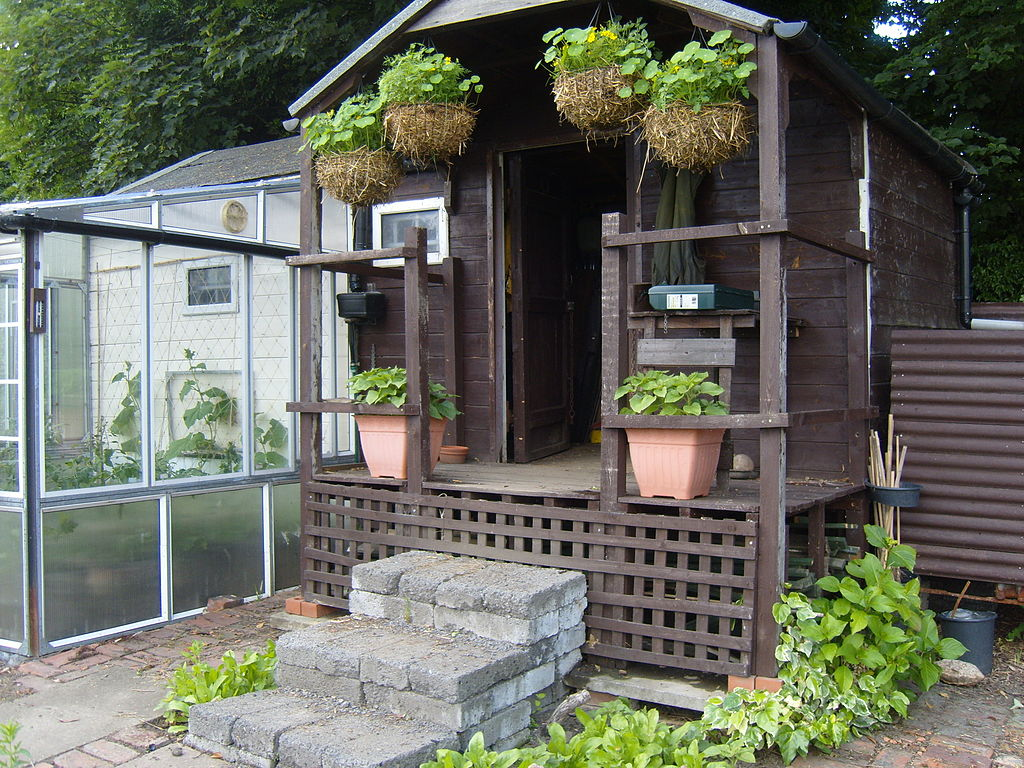
\includegraphics[width=0.5\textwidth]{images/Gartenhaus.jpg}
	\caption[Bild eines Gartenhauses.]{Bild eines Gartenhauses.
		Das Gartenhaus ist frei stehend und mit hängenden Pflanzen beschmückt.\footnotemark
	}
	\label{pic:gartenhaus}
\end{figure}

\footnotetext{Bildquelle: Allotmenteer, \href{https://creativecommons.org/licenses/by-sa/3.0}{CC BY-SA 3.0}, via Wikimedia Commons}

Ein Gartenhaus ist wie in \cref{pic:gartenhaus} zu sehen eine frei stehende Struktur im Garten, welche als Lagerplatz für Gartengeräte, Werkzeuge und andere Utensilien genutzt wird.
Außerdem kann es als Arbeitsbereich für Gartenarbeit, Bastelprojekte oder als Rückzugsort dienen.
Viele Objekte, die in einem Gartenhaus gelagert werden, sind anfällig für Frost und Feuchtigkeit, weshalb Messungen von Temperatur und Luftfeuchtigkeit in einem Gartenhaus sinnvoll sind, wofür auch Wetterdaten hilfreich sein können.
Durch diese Messungen kann der Nutzer informiert werden, wenn die Werte kritisch werden, damit er rechtzeitig Gegenmaßnahmen einleiten kann.
Diese könnten etwa das Heizen des Gartenhauses oder das Entfernen betroffener Gegenstände sein.
Für Gegenstände in der Hütte kann ein intelligentes Regalsystem eingesetzt werden, wofür sich Technologien wie RFID-Tags eignen.
Dadurch kann der Nutzer schnell und einfach Gegenstände finden und verwalten.

\subsubsection{Gartenelement Gehege / Stall}
\begin{figure}[!htb]
	\centering
	\includegraphics[width=0.5\textwidth]{images/Hühnerstall.jpg}
	\caption[Bild eines Hühnerstalls in einem Gehege.]{
		Bild eines Hühnerstalls in einem Gehege.
		Der Stall ist frei stehend und das Gehege ist von einem großen Zaun umgeben.\footnotemark
	}
	\label{pic:stall}
\end{figure}

So wie in \cref{pic:stall} zu sehen ist ein Gehege ein abgegrenzter Bereich im Garten, der der Haltung von Tieren dient und ein Stall ist ein Gebäude, in dem Tiere gehalten werden.
Beide können für die Haltung verschiedener Tiere genutzt werden.
So gibt es Gehege und Ställe für Hühner, Kaninchen, Meerschweinchen, Vögel, Schildkröten und viele andere Tiere.
Diese Tiere benötigen regelmäßige Pflege, wie das Füttern, das Tränken und das Reinigen des Geheges oder Stalls.
Für das Füttern und Tränken können regelbasierte Fütterungssysteme und Tränksysteme eingesetzt werden.
Die Tiere haben außerdem Anforderungen an die Temperatur.
Durch Temperaturmessungen in Kombination mit Wetterdaten kann der Nutzer informiert werden, wenn es zu kalt oder zu warm wird.
So kann der Nutzer rechtzeitig Gegenmaßnahmen einleiten, um die Tiere zu schützen.
Wassernäpfe frieren etwa bei Frost ein, weshalb der Nutzer in diesen Fällen reagieren muss oder eine automatische Wasserenteisung eingesetzt werden kann.
In Ställen kann auch die Luftqualität eine wichtige Rolle spielen, die sich aus CO$_2$-Konzentration und Luftfeuchtigkeit sowie der Temperatur zusammensetzt.
Durch Messungen dieser Werte kann eine automatische Lüftung gesteuert werden.
\footnotetext{Bildquelle: Phil Catterall, \href{https://creativecommons.org/licenses/by-sa/2.0}{CC BY-SA 2.0}, via Wikimedia Commons}

\subsubsection{Gartenelement Bienenstock}
Ein Bienenstock ist eine Struktur, die von Imkern verwendet wird, um Bienen zu züchten und Honig zu produzieren.
Wie in \cref{pic:bienenstock} zu sehen, bestehen Bienenstöcke aus mehreren Elementen, den Bienenkästen, in denen sich Rahmen und Waben befinden.
Diese Bienenkästen haben unterschiedliche Funktionen, wie Brutraum, Honigraum und Futterraum.
Der unterste Kasten hat den Eingang für die Bienen.
Diese Kästen bieten den Bienen Lebensraum und Platz zur Nestbildung und dem Lagern von Honig.

\begin{figure}[!htb]
	\centering
	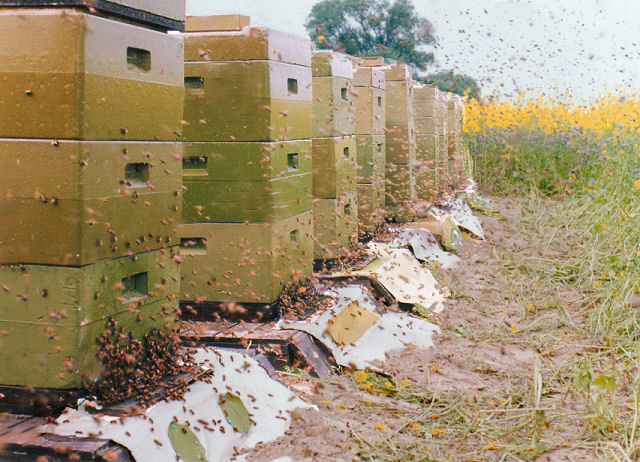
\includegraphics[width=0.5\textwidth]{images/Bienenstock.jpg}
	\caption[Bild mehrerer Bienenstöcke.]{
		Bild mehrerer Bienenstöcke.
		Die Bienen fliegen vor den Bienenstöcken herum.
		Der Eingang für die Bienen befindet sich unten.\footnotemark
	}
	\label{pic:bienenstock}
\end{figure}

\footnotetext{Bildquelle: Axel Hindemith, Public Domain, via Wikimedia Commons}

Bienenstöcke benötigen regelmäßige Pflege, wozu das Füttern, das Überwachen des Bienenstocks und das Ernten des Honigs gehören.
Insbesondere bei der Überwachung des Bienenstocks kann Technik dem Imker helfen.
So kann eine dauerhafte Überwachung des Gewichts des Bienenstocks dem Imker wertvolle Informationen geben~\cite{BienenGewicht}.
Beispielsweise kann ein erhöhter Futterverbrauch am Gewicht abgelesen werden, welcher auf eine Krankheit oder Parasitenbefall hindeuten kann.
Gibt es solche unerwarteten Schwankungen, kann der Imker informiert werden, damit er reagieren kann.
Auch der Futterstand kann damit überwacht werden, da insbesondere im Winter eine Notfütterung nötig werden kann.

Eine weitere wichtige Information für den Imker ist der Status der Bienenkönigin.
Wenn das Volk eine neue Bienenkönigin heranzieht, so zieht die Alte mit einem Teil des Volkes aus, was als Schwärmen bezeichnet wird.
Dies möchte der Imker verhindern, da er dadurch einen Teil seines Volkes verliert.
Auch muss die Bienenkönigin innerhalb der Bienenmasse gefunden werden können.
Wie in \cref{pic:bienenstock} zu sehen, haben die einzelnen Kästen Griffe, die es ermöglichen, die Kästen zu heben.
Die Königin befindet sich in einem dieser Kästen zwischen den Rahmen und anderen Bienen, weshalb die Nutzung von Technik wie RFID-Tags helfen kann, die Königin zu finden.

Die Temperatur im Bienenstock ist ebenfalls ein wichtiger Wert, da der Imker anhand Temperaturänderungen verschiedene Ereignisse im Bienenstock erkennen kann~\cite{BienenTemperatur}.
Auch die Luftfeuchtigkeit ist ein wichtiger Wert für einen Imker, da eine zu niedrige Luftfeuchtigkeit die Brut austrocknen und eine zu hohe Luftfeuchtigkeit den Bienenstock schimmeln lassen kann~\cite{BienenLuftfeuchtigkeit}.

\subsubsection{Gartenelement Kompost}
\begin{figure}[!htb]
	\centering
	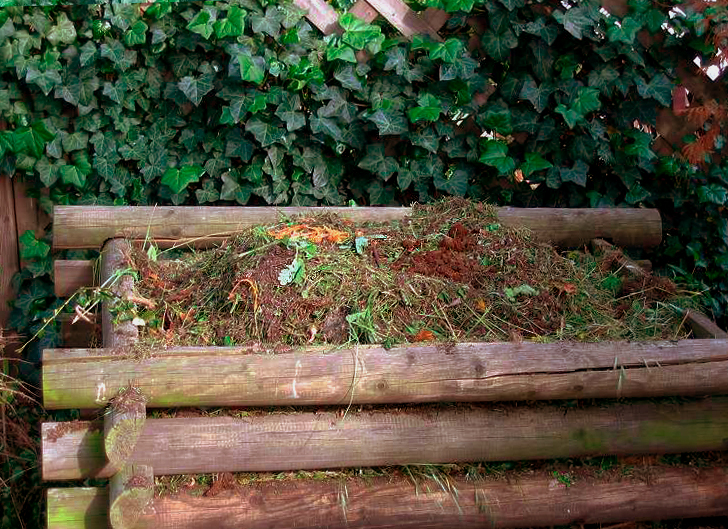
\includegraphics[width=0.5\textwidth]{images/Kompost.jpg}
	\caption[Bild eines Komposthaufens.]{
		Bild eines Komposthaufens.
		Der Kompost besteht aus verschiedenen Elementen, die durch die unterschiedlichen Farben erkennbar sind.\footnotemark
	}
	\label{pic:kompost}
\end{figure}
\footnotetext{Bildquelle: Mussklprozz, \href{https://creativecommons.org/licenses/by-sa/3.0}{CC BY-SA 3.0}, via Wikimedia Commons}
Kompost entsteht durch die Zersetzung von Garten- und Küchenabfällen sowie anderen organischen Materialien wie Laub, Gras und Papierschnipseln.
Das Ergebnis ist ein nährstoffreicher Humus, der als Dünger im Garten eingesetzt werden kann.
Der Prozess der Kompostierung durchläuft dabei mehrere Phasen, nämlich die Vorrotte, Heißrotte, Hauptrotte und Nachrotte.
Gleichzeitig erfordert Kompostierung Aufmerksamkeit und Pflege, um optimale Bedingungen für die Zersetzung zu schaffen.
Diese Bedingungen umfassen die richtige Mischung von grünen (stickstoffreichen) und braunen (kohlenstoffreichen) Materialien, ausreichende Feuchtigkeit und regelmäßige Belüftung~\cite{Kompost}.
Dies ist in \cref{pic:kompost} ersichtlich, wo man den lockeren Komposthaufen mit braunen und grünen Materialien sieht.
Weitergehend unterstützt eine Überwachung der Werte Kohlenstoff, Stickstoff, Feuchtigkeit und ph-Wert den Nutzer bei der Pflege des Kompostes.
Auch die Sicherheit ist ein wichtiger Aspekt, da Kompostierungsprozesse durch die entstehende Wärme zu Bränden führen können.
Außerdem beeinflusst die Temperatur die Belüftungszeiten, die für den Kompostierungsprozess wichtig sind.
Daher ist es wichtig, die Temperatur im Komposthaufen zu überwachen, sodass der Nutzer informiert wird, wenn die Temperatur zu hoch oder zu niedrig ist.
Parameter wie die Temperatur, Zusammensetzung und Feuchtigkeit des Kompostes bestimmen die Geschwindigkeit der Zersetzung und die Qualität des Kompostes.
Daher unterstützt die Überwachung dieser Parameter den Nutzer bei der Pflege des Kompostes.


\subsubsection{Zusammenfassung der Gartenelemente}
Gerade wurde die Vielfalt der verschiedenen Gartenelemente dargestellt
Diese Liste ist nicht vollständig und kann es auch nicht sein, deckt aber die häufigsten Elemente ab.
Andere Elemente können als Unterarten oder Kombinationen dieser Elemente betrachtet werden.
So ist etwa ein Planschbecken ein kleiner Pool ohne Pumpe und Filter oder ein Hochbeet eine Art Beet mit einem erhöhten Bedarf nach Bewässerung.
Alle Gartenelemente können in verschiedenen Arten von Smart Gardening Lösungen profitieren, wobei die Anforderungen an diese unterschiedlich sind.
Hierbei kann es sich beispielsweise um Arbeitserleichterungen, Kosteneinsparungen oder Ertragssteigerungen handeln.
\pagebreak
\begin{table}[!h]
	\centering
	\caption[Gegenüberstellung von Gartenelementen: relevante Messwerte.]{
		Gegenüberstellung verschiedener Gartenelemente basierend auf den relevanten Messwerten.
		In den Zeilen sind die verschiedenen Gartenelemente aufgelistet und in den Spalten die verschiedenen Messwerte.
		Messwerte, die für das jeweilige Gartenelement relevant sind, sind mit einem Häkchen markiert und Messwerte, die nicht relevant sind, mit einem Kreuz.
		Einige Messwerte sind nur für wenige Gartenelemente relevant.
		Diese Elemente sind für die Übersichtlichkeit in der Tabelle als \emph{Andere} enthalten.
		Das betrifft folgende Messwert-Gartenelement-Kombinationen:
		Ammoniumstickstoff und Sauerstoff für Gartenteich, Chlor, Cyansäure, Redox und Alkalinität für Pool, CO$_2$ für Gewächshaus und Gehege/Stall.
		}\label{tab:gartenelementemessungen}
	\begin{tabular}{lllllllllllll}
		\rot[\tabellenwinkel]{				} &
		\rot[\tabellenwinkel]{Temperatur	} &
		\rot[\tabellenwinkel]{Wetter		} &
		\rot[\tabellenwinkel]{Feuchtigkeit	} &
		\rot[\tabellenwinkel]{Schädlinge	} &
		\rot[\tabellenwinkel]{Stickstoff	} &
		\rot[\tabellenwinkel]{Phosphor		} &
		\rot[\tabellenwinkel]{Licht			} &
		\rot[\tabellenwinkel]{Pegel			} &
		\rot[\tabellenwinkel]{Gewicht		} &
		\rot[\tabellenwinkel]{RFID			} &
		\rot[\tabellenwinkel]{pH-Wert		} &
		\rot[\tabellenwinkel]{Andere		}\\\hline
		Rasen					& \OK & \NO & \OK & \OK & \OK & \OK & \NO & \NO & \NO & \NO & \NO & \NO \\
		Beet					& \OK & \OK & \OK & \OK & \OK & \OK & \NO & \NO & \NO & \NO & \NO & \NO \\
		Baum					& \NO & \OK & \OK & \NO & \OK & \NO & \NO & \NO & \NO & \NO & \NO & \NO \\
		Pflanzentopf			& \OK & \OK & \OK & \OK & \OK & \OK & \OK & \NO & \NO & \NO & \NO & \NO \\
		Gewächshaus				& \OK & \OK & \OK & \OK & \OK & \OK & \OK & \NO & \NO & \OK & \NO & \OK \\[.2cm]
		Regentonne				& \OK & \OK & \NO & \NO & \NO & \NO & \NO & \OK & \NO & \NO & \NO & \NO \\
		Brunnen					& \OK & \OK & \NO & \NO & \NO & \NO & \NO & \NO & \OK & \NO & \NO & \NO \\
		Gartenteich				& \OK & \OK & \NO & \OK & \OK & \NO & \NO & \OK & \NO & \NO & \OK & \OK \\
		Pool					& \OK & \OK & \NO & \NO & \NO & \NO & \NO & \NO & \NO & \NO & \OK & \OK \\[.2cm]
		Gartenhaus				& \OK & \OK & \OK & \NO & \NO & \NO & \NO & \NO & \NO & \OK & \NO & \NO \\[.2cm]
		Gehege / Stall			& \OK & \OK & \OK & \NO & \NO & \NO & \NO & \NO & \NO & \NO & \NO & \OK \\
		Bienenstock				& \OK & \NO & \OK & \OK & \NO & \NO & \NO & \NO & \OK & \OK & \NO & \NO \\[.2cm]
		Kompost					& \OK & \NO & \OK & \NO & \OK & \OK & \NO & \NO & \NO & \NO & \OK & \NO \\
	\end{tabular}
\end{table}

Bei den verschiedenen Gartenelementen können unterschiedlichen Messungen sinnvoll eingesetzt werden, wobei die jeweiligen relevanten Messwerte in \cref{tab:gartenelementemessungen} dargestellt sind.
Dabei gibt es einige Gemeinsamkeiten, so profitieren die meisten Gartenelemente von Temperaturmessungen und Wetterdaten.
Weiterhin teilen sich die Gartenelemente, die Pflanzen enthalten, die meisten Messwerte, mit wenigen Ausnahmen.
Dies erklärt sich dadurch, dass Pflanzen ähnliche Bedürfnisse haben und diese Messwerte für die Pflege wichtig sind.
Einige Messwerte sind jedoch nur für wenige der betrachteten Gartenelemente relevant, wie die Pegelmessung und die Gewichtsmessung.

Die für die Gartenelemente relevanten Aktionen sind in \cref{tab:gartenelementeaktuatoren} dargestellt.
Dabei gibt es einige Gemeinsamkeiten, so profitieren alle betrachteten Gartenelemente von der Möglichkeit den Nutzer zu benachrichtigen.
Weiterhin teilen sich die Gartenelemente, die Pflanzen enthalten, die meisten Aktionen, mit wenigen Ausnahmen.
Dies erklärt sich dadurch, dass Pflanzen ähnliche Bedürfnisse haben und diese Aktionen für die Pflege wichtig sind.
Die nicht pflanzenhaltenden Gartenelemente haben dabei sehr unterschiedliche Anforderungen an die Aktionen, wie in der Tabelle ersichtlich.

Aus der kombinierten Betrachtung der Messungen und Aktionen ist ersichtlich, dass ein Fokus auf die pflanzenhaltenden Gartenelemente sinnvoll ist, da diese die meisten Messungen und Aktionen teilen.


\begin{table}[!htb]
	\centering
	\caption[Gegenüberstellung von Gartenelementen: relevanten Aktionen.]{
		Gegenüberstellung verschiedener Gartenelemente basierend auf den relevanten Aktionen des Smart Gardening Systems.
		In den Zeilen sind die verschiedenen Gartenelemente aufgelistet und in den Spalten die verschiedenen Aktionen.
		Aktionen, die für das jeweilige Gartenelement relevant sind, sind mit einem Häkchen markiert und Aktionen, die nicht relevant sind, mit einem Kreuz.
		}\label{tab:gartenelementeaktuatoren}
	\begin{tabular}{llllllllllll}
		\rot[\tabellenwinkel]{						} &
		\rot[\tabellenwinkel]{Benachrichtigung		} &
		\rot[\tabellenwinkel]{Bewässerung			} &
		\rot[\tabellenwinkel]{Düngung				} &
		\rot[\tabellenwinkel]{Schädlinge			} &
		\rot[\tabellenwinkel]{Fütterung				} &
		\rot[\tabellenwinkel]{Tränkung				} &
		\rot[\tabellenwinkel]{Wasserqualität		} &
		\rot[\tabellenwinkel]{Lüftung				} &
		\rot[\tabellenwinkel]{Luftbe-/entfeuchtung	} &
		\rot[\tabellenwinkel]{Heizung				} \\\hline
		Rasen					& \OK & \OK & \OK & \OK & \NO & \NO & \NO & \NO & \NO & \NO \\
		Beet					& \OK & \OK & \OK & \OK & \NO & \NO & \NO & \NO & \NO & \NO \\
		Baum					& \OK & \OK & \NO & \OK & \NO & \NO & \NO & \NO & \NO & \NO \\
		Pflanzentopf			& \OK & \OK & \OK & \OK & \NO & \NO & \NO & \NO & \NO & \NO \\
		Gewächshaus				& \OK & \OK & \OK & \OK & \NO & \NO & \NO & \OK & \OK & \OK \\[.2cm]
		Regentonne				& \OK & \OK & \NO & \NO & \NO & \NO & \NO & \NO & \NO & \NO \\
		Brunnen					& \OK & \OK & \NO & \NO & \NO & \NO & \NO & \NO & \NO & \NO \\
		Gartenteich				& \OK & \NO & \NO & \OK & \OK & \NO & \OK & \NO & \NO & \NO \\
		Pool					& \OK & \NO & \NO & \NO & \NO & \NO & \OK & \NO & \NO & \NO \\[.2cm]
		Gartenhaus				& \OK & \NO & \NO & \NO & \NO & \NO & \NO & \NO & \NO & \NO \\[.2cm]
		Gehege / Stall			& \OK & \NO & \NO & \NO & \OK & \OK & \NO & \OK & \OK & \OK \\
		Bienenstock				& \OK & \NO & \NO & \NO & \NO & \NO & \NO & \NO & \NO & \NO \\[.2cm]
		Kompost					& \OK & \NO & \NO & \NO & \NO & \NO & \NO & \NO & \NO & \NO \\
	\end{tabular}
\end{table}


\subsection{Zusammenfassung Kontext und Umfeld}
In diesem Abschnitt wurden verschiedene Gartenarten und Gartenelemente betrachtet.
Diese weisen unterschiedliche Bedarfe an die Pflege und Überwachung auf, die durch Smart Gardening unterstützt werden können.
Dazu gehören unter anderem automatische Bewässerungs- und Düngesysteme sowie Warnsysteme für Situationen wie Frost oder Schädlinge, in denen der Nutzer eingreifen muss.
Die für ein solches System benötigten Messungen und Aktionen sind unter anderem Temperaturmessungen, Wetterdaten, Feuchtigkeitsmessungen, Schädlingsüberwachung, Bewässerung, Düngung, Fütterung, Tränkung, Überwachung der Wasserqualität, Lüftung, Luftbe- und -entfeuchtung und Heizung.
Daraus folgt, dass ein universelles Sensor- und Aktuatorsystem für Smart Gardening eine Vielzahl von Sensoren und Aktuatoren unterstützen muss.

Gleichzeitig können die Gartenelemente in verschiedenen Kombinationen mit unterschiedlichen Gartenarten auftreten, welche in \cref{tab:gartenelementeartenmapping} dargestellt sind.
Dabei wird ersichtlich, dass einige Gartenarten praktisch alle betrachteten Gartenelemente enthalten können, während andere nur wenige enthalten.
Hierbei ähneln sich der Balkongarten und das Gewächshaus, die jeweils nur drei der betrachteten Elemente enthalten können, während der Kleingarten und Hintergarten jeweils alle der betrachteten Elemente enthalten können.
Auch der Vorgarten und der Landschaftsgarten ähneln sich, was hauptsächlich an dem ähnlichen Zweck der Außenwirkung liegt.

\begin{table}[!htb]
	\centering
	\caption[Kombinationsmöglichkeiten von Gartenarten und Gartenelementen.]{
		Darstellung der verschiedenen Möglichkeiten, Gartenarten und Gartenelemente zu kombinieren.
		In den Zeilen sind die verschiedenen Gartenelemente aufgelistet und in den Spalten die verschiedenen Gartenarten.
		Die Kombinationen, die in der Praxis vorkommen können, sind mit einem Häkchen markiert und die Kombinationen, die nicht vorkommen, mit einem Kreuz.
		}\label{tab:gartenelementeartenmapping}
	\begin{tabular}{lllllllll}
		\rot[\tabellenwinkel]{					} &
		\rot[\tabellenwinkel]{Balkongarten		} &
		\rot[\tabellenwinkel]{Gewächshaus		} &
		\rot[\tabellenwinkel]{Vorgarten			} &
		\rot[\tabellenwinkel]{Kleingarten		} &
		\rot[\tabellenwinkel]{Hintergarten		} &
		\rot[\tabellenwinkel]{Landschaftsgarten	} &
		\rot[\tabellenwinkel]{Landwirtschaft	}\\\hline
		Rasen					& \NO & \NO & \OK & \OK & \OK & \OK & \OK \\
		Beet					& \NO & \NO & \OK & \OK & \OK & \OK & \NO \\
		Baum					& \NO & \NO & \OK & \OK & \OK & \OK & \OK \\
		Pflanzentopf			& \OK & \OK & \OK & \OK & \OK & \NO & \NO \\
		Gewächshaus				& \OK & \OK & \NO & \OK & \OK & \NO & \NO \\[.2cm]
		Regentonne				& \OK & \OK & \OK & \OK & \OK & \NO & \NO \\
		Brunnen					& \NO & \NO & \OK & \OK & \OK & \OK & \OK \\
		Gartenteich				& \NO & \NO & \OK & \OK & \OK & \OK & \NO \\
		Pool					& \NO & \NO & \NO & \OK & \OK & \NO & \NO \\[.2cm]
		Gartenhaus				& \NO & \NO & \NO & \OK & \OK & \NO & \NO \\[.2cm]
		Gehege / Stall			& \NO & \NO & \NO & \OK & \OK & \NO & \OK \\
		Bienenstock				& \NO & \NO & \NO & \OK & \OK & \OK & \OK \\[.2cm]
		Kompost					& \NO & \NO & \OK & \OK & \OK & \NO & \NO \\
	\end{tabular}
\end{table}



\section{Anforderungen}
In diesem Abschnitt werden Anforderungen an ein universelles Sensor- und Aktuatorsystem für Smart Gardening definiert.
Dabei wird auf die Definition von Smart Gardening, die Zielgruppe und die Anwendungsfälle in den Gartenarten und Gartenelementen eingegangen.
Das System soll potenziell alle der oben genannten Anwendungsfälle für die definierte Zielgruppe abdecken können.
Im Folgenden werden dabei zunächst die funktionalen Anforderungen und anschließend die nicht funktionalen Anforderungen betrachtet.


\subsection{Funktionale Anforderungen}
In diesem Abschnitt werden die funktionalen Anforderungen an das System betrachtet, welche beschreiben, was das System leisten soll und was das System benötigt, um diese Leistungen zu erbringen.
In der vorherigen Analyse der Gartenarten und Gartenelemente wurden einige Anforderungen an das System bereits implizit genannt, wie die Notwendigkeit für Sensorik, um Messungen der Umgebung durchzuführen.
In der Analyse wurden bereits einige Messwerte genannt, die für ein Smart Gardening System relevant sind, welche in der \cref{tab:gartenelementemessungen} zusammengefasst sind, wie die Temperatur, die Feuchtigkeit, der Stickstoffgehalt und der pH-Wert.
Diese Liste ist nicht vollständig, sondern deckt nur die häufigsten Nutzungsszenarien ab.
Allein in dieser Auflistung sind bereits 19 Messwerte enthalten, die jeweils nur in bestimmten Szenarien relevant sind.
Die Messung des CO$_2$-Gehalts ist beispielsweise nur im Gewächshaus und im Stall von Interesse.
An dieser Stelle kann die Vielfalt der Sensoren und Sensorschnittstellen nicht abgegrenzt werden, weshalb das System modular sein sollte.
Es sollte möglich sein, Sensoren hinzuzufügen oder zu entfernen.
Da viele Sensoren unterschiedliche Schnittstellen haben, sollten möglichst viele Schnittstellen unterstützt werden, wie I2C, SPI, UART, Modbus und 1-Wire. 

Das System benötigt auch Aktuatorik, um Aktionen durchzuführen.
In der Analyse wurden bereits einige Aktionen genannt, die für ein Smart Gardening System relevant sind, welche in der \cref{tab:gartenelementeaktuatoren} zusammengefasst sind.
Dazu gehören etwa die Bewässerung, die Düngung, die Fütterung und die Tränkung, wobei auch hier einige Aktionen nur in bestimmten Szenarien relevant sind.
Außerdem sieht beispielsweise die Steuerung der Bewässerung für einen Rasen anders aus als für ein Gewächshaus.
Es besteht also ein Bedarf an einer Vielfalt von Aktuatoren, weshalb auch dieser Teil des Systems modular sein sollte.
Es sollte möglich sein, Aktuatoren hinzuzufügen oder zu entfernen.

Weiterhin ist es wichtig, dass das System den Nutzer über wichtige Ereignisse über eine definierbare Schnittstelle wie E-Mail, SMS oder Push-Benachrichtigung benachrichtigen kann.
Dabei soll der Nutzer nicht über jeden kleinen Schritt, sondern nur über besonders wichtige Informationen direkt informiert werden, wozu unter anderem kritische Messwerte oder Aktionen gehören.

Ein weiterer wichtiger Aspekt ist die Möglichkeit der Fernüberwachung.
Regelmäßige Messungen und Aktionen sollen in einem Dashboard zusammengefasst und in einem digitalen Zwilling des Gartens und der Gartenelemente modelliert werden.
Darauf aufbauend wird als weitere Anforderung eine Netzwerkfähigkeit benötigt.
Das System soll in der Lage sein, mit dem Netzwerk zu kommunizieren, wozu die Übertragung der Messwerte, Aktionen und Benachrichtigungen gehört.
Genauer benötigt das System eine LAN und WAN Schnittstelle.

Auch die Konfigurierbarkeit des Systems bezogen auf das Zusammenspiel der Sensoren, Aktuatoren und Benachrichtigungen ist eine wichtige Anforderung.
Diese Konfiguration soll möglichst einfach und intuitiv sein, aber auch komplexere Konfigurationen ermöglichen.
Hierbei ist die grundlegende Möglichkeit der Integration unterschiedlicher Sensoren, Aktuatoren und Benachrichtigungen wichtig.

Aufbauend auf der Konfigurierbarkeit ist die Möglichkeit der Regeldefinition, um das System automatisiert steuern zu können, eine weitere wichtige Anforderung.
So soll es möglich sein, Regeln zu definieren, welche bestimmte Aktionen auslösen können, wenn bestimmte Bedingungen erfüllt sind.
Die Definition folgender Beispielregel soll möglich sein:
\begin{enumerate}
	\item Der Rasen wird bewässert, wenn die Temperatur über 30 Grad steigt.
	\item Der Nutzer wird benachrichtigt.
\end{enumerate}

Ein weiterer wichtiger Aspekt ist die Stromversorgung, da viele Gärten und Gartenelemente existieren, die nicht in der Nähe einer Steckdose liegen.
Daher muss das System in solchen Fällen autonom arbeiten können, was beispielsweise durch Solarzellen oder Akkus erfolgen kann.
Gleichzeitig soll das System in diesem autonomen Zustand möglichst selten aufgeladen werden müssen, weshalb ein geringer Energieverbrauch wichtig ist.
Auch eine fest installierte Wasserversorgung ist nicht immer gegeben.
Daher sollte das System auch mit einer Regentonne oder einem Brunnen arbeiten können.

Zusammengefasst soll das System den folgenden funktionalen Anforderungen genügen, die hierbei nach ihrer Wichtigkeit sortiert sind:
\begin{itemize}
	\item Messung mittels Sensoren
	\item Konfiguration des Systems
	\item Regeldefinition
	\item Dashboard mit digitalem Zwilling basierend auf den Messwerten und Aktionen
	\item Steuerung von Aktuatoren
	\item Autonomer Betrieb
	\item Benachrichtigung des Nutzers
\end{itemize}
Diese Reihenfolge ergibt sich aus der Annahme, dass die Messung der Umgebung die Grundlage für alle weiteren Funktionen bildet.
Die Konfiguration des Systems ist wichtig, um das System an die individuellen Bedürfnisse des Nutzers anzupassen und daran anschließend die Regeldefinition, um das System automatisiert steuern zu können.
Ein Dashboard mit digitalem Zwilling ist wichtig, um dem Nutzer einen Überblick über den Zustand des Gartens zu geben.
Die Steuerung von Aktuatoren ist in der Priorität hinter der Sensorik, da die Sensorik die Grundlage für die Steuerung bildet und viele Anwendungsfälle ohne Aktuatoren auskommen können.
Der autonome Betrieb ist wichtig, um das System auch in Gärten ohne Strom- und Wasserversorgung einsetzen zu können und eine Benachrichtigung des Nutzers ist wichtig, um den Nutzer über wichtige Ereignisse zu informieren.



\subsection{Nicht funktionale Anforderungen}
In diesem Abschnitt werden die nicht funktionalen Anforderungen an das System betrachtet, welche beschreiben, wie das System arbeiten soll.
Dabei sind die nicht funktionalen Anforderungen nach ihrer Wichtigkeit sortiert.

An erster Stelle steht der Preis des Systems.
Da die primäre Zielgruppe Hobbygärtner und somit Privatpersonen mit begrenztem Budget sind, sollte das System möglichst günstig sein.
Auch der Energieverbrauch und die Wartung des Systems sind Faktoren, die den Preis beeinflussen.

Weiterer wichtiger Punkt ist der Schutz beziehungsweise die Resilienz des Systems vor den Elementen.
Das System muss wasserfest, dreckfest, robust und temperaturbeständig sein, sowie fest installierbar, damit es nicht vom Wind weggeweht werden kann.
Für den Wasser- und Staubschutz gibt es die IP Schutzart, wobei für einen universellen Einsatz im Garten IP Schutzklasse 6 staubdicht und Schutzgrad 8 geschützt vor andauerndem Untertauchen, also IP68 sinnvoll ist.
Auch die Sonne mit ihren UV-Strahlen kann dem System schaden, weshalb es vor der Sonne geschützt werden muss~\cite{LichtPlastik,LichtPlastik2}.

Auch die Bedienung des Systems soll nutzerfreundlich sein.
Der Nutzer soll nicht lange brauchen, um das System zu bedienen, es sollte also eine flache Lernkurve haben.
Dies ist insbesondere wichtig, da vor allem Hobbygärtner das System nutzen werden.

Ein weiterer wichtiger Aspekt ist die Sicherheit des Systems.
Das Smart Gardening System ist mit Sensorik ausgestattet, welche Daten über den Garten und Umgebung erheben.
Kommt ein Angreifer in Besitz dieser Daten, können sie potenziell ausgenutzt werden.
Sie können beispielsweise genutzt werden, um das Verhalten der Bewohner zu analysieren, in das Haus einzubrechen oder den Garten zu zerstören.
Da die Messdaten oder Auswertungen dieser Messdaten über ein Netzwerk übertragen werden, ist eine sichere Übertragung wichtig, beispielsweise durch Verschlüsselung der Daten.
Weiter dürfen die Daten bei der Übertragung nicht geändert werden, die Datenintegrität muss also gewährleistet sein.
Des Weiteren ist auch ein Angriff auf die Aktuatorik denkbar.
Ein Angreifer könnte etwa die Bewässerung des Gartens manipulieren, wenn das System eine Fernsteuerung zulässt.
Daher darf die Aktuatorik nur von authentifizierten Nutzern gesteuert werden.
Das Gleiche gilt auch, wenn das Smart Gardening System von Landwirten oder Gärtnern eingesetzt wird.

Ein sparsamer Energieverbrauch ist aus zwei Gründen wichtig.
Zum einen hat der Energieverbrauch einen Einfluss auf den Preis des Systems, da ein höherer Energieverbrauch auch höhere Betriebskosten bedeutet.
Zum anderen ist ein sparsamer Energieverbrauch wichtig, wenn das System auch unabhängig vom Stromnetz betrieben werden können soll.

Auch die Verfügbarkeit des Systems ist wichtig, da ein unerkannter Ausfall des Systems zu Schäden im Garten führen kann.
Da die Verfügbarkeit nicht garantiert werden kann, muss der Nutzer im Fehlerfall informiert werden.

Die Wartbarkeit des Systems ist ein weiterer wichtiger Aspekt.
Das System soll möglichst einfach wartbar sein, damit der Nutzer es selbst warten kann.
Dazu gehört beispielsweise, dass das System modular aufgebaut ist, sodass defekte Sensoren oder Aktuatoren einfach ausgetauscht werden können.

Weiterhin soll das System möglichst unauffällig sein, was insbesondere für Vorgärten wichtig ist, die von der Straße aus einsehbar sind.
Dazu gehört, dass es nicht zu groß ist und sich in die Umgebung integrieren lässt.

Zusammengefasst soll das System diesen nicht funktionalen Anforderungen genügen:
\begin{itemize}
	\item Preis
	\item Schutz vor den Elementen
	\item Nutzerfreundliche Bedienung
	\item Sicherheit (Datenintegrität, Datenschutz, Angriffssicherheit)
	\item Sparsamer Energieverbrauch
	\item Verfügbarkeit des Systems
	\item Einfache Wartbarkeit
	\item Visuelle Unauffälligkeit
\end{itemize}

\subsection{Zusammenfassung der Anforderungen}
In diesem Abschnitt wurden die funktionalen und nicht funktionalen Anforderungen an ein universelles Sensor- und Aktuatorsystem für Smart Gardening definiert.
Diese Anforderungen wurden auf Basis der Definition von Smart Gardening, der Zielgruppe und der Anwendungsfälle in den Gartenarten und Gartenelementen erarbeitet.

Die funktionalen Anforderungen beschreiben, was das System leisten soll und was das System benötigt, um diese Leistungen zu erbringen.
Dabei wurden die Messung mittels Sensoren, die Steuerung von Aktuatoren, die Benachrichtigung des Nutzers, die Konfiguration des Systems, die Regeldefinition, ein Dashboard mit digitalem Zwilling basierend auf den Messwerten und Aktionen und der autonome Betrieb als funktionalen Anforderungen definiert.

Die nicht funktionalen Anforderungen beschreiben, wie das System arbeiten soll.
Dabei wurden die Sicherheit, die Verfügbarkeit des Systems, der Preis, der sparsame Energieverbrauch, die einfache Wartbarkeit, der Schutz vor den Elementen, die visuelle Unauffälligkeit und die nutzerfreundliche Bedienung als nicht funktionale Anforderungen definiert.



\section{Zusammenfassung der Analyse}
In diesem Kapitel wurde der Einsatz von Smart Gardening im Garten analysiert.
Die Zielgruppe besteht vorrangig aus Gärtnern, unterteilt in Hobbygärtner und professionelle Gärtner sowie nachrangig Landwirte.
Smart Gardening kann in verschiedenen Gartenarten und Gartenelementen eingesetzt werden.
Dabei wurden die Gartenarten Balkongarten, Gewächshaus, Vorgarten, Kleingarten, Hintergarten, Landschaftsgarten und zusätzlich die Landwirtschaft betrachtet.
Hier können Smart Gardening Lösungen etwa Arbeitserleichterungen, Kosteneinsparungen oder Ertragssteigerungen bringen.
Gleichzeitig stellen die Strom-, Wasser- und Internetversorgung für das Smart Gardening System eine Herausforderung dar.
Als Gartenelemente wurden Rasen, Beet, Baum, Pflanzentopf, Gewächshaus, Regentonne, Brunnen, Gartenteich, Pool, Gartenhaus, Gehege/Stall, Bienenstock und Kompost betrachtet.

Darauf aufbauend wurden Anforderungen an ein universelles Sensor- und Aktuatorsystem für Smart Gardening definiert.
Zu den funktionalen Anforderungen gehören die Messung mittels Sensoren, die Steuerung von Aktuatoren, die Benachrichtigung des Nutzers, die Konfiguration des Systems, die Regeldefinition, ein Dashboard mit digitalem Zwilling basierend auf den Messwerten und Aktionen und der autonome Betrieb.
Zu den nicht funktionalen Anforderungen gehören die Sicherheit, die Verfügbarkeit des Systems, der Preis, der sparsame Energieverbrauch, die einfache Wartbarkeit, der Schutz vor den Elementen, die visuelle Unauffälligkeit und die nutzerfreundliche Bedienung.
Basierend auf diesen Anforderungen wird im nächsten Kapitel der Stand der Technik betrachtet, um zu sehen, inwieweit existierende Systeme diesen Anforderungen genügen.